\documentclass[12pt,a4paper]{report}

% -------------------------------
% PACKAGES
% -------------------------------
\usepackage[T1]{fontenc}
\usepackage[utf8]{inputenc}
\usepackage{lmodern}
\usepackage{setspace}
\usepackage{microtype}
\usepackage{graphicx}
\usepackage{amsmath, amssymb}
\usepackage{hyperref}
\usepackage{caption}
\usepackage{subcaption}
\usepackage{booktabs}
\usepackage{url}
\usepackage{enumitem}
\usepackage{float}
\usepackage{algorithm}
\usepackage{algpseudocode}
\usepackage{tikz}
\usetikzlibrary{shapes.geometric, arrows.meta, positioning}

\usepackage[a4paper,margin=1in]{geometry}

% Chapter style similar to thesis PDF
\usepackage{titlesec}
\titleformat{\chapter}[hang]
  {\bfseries\huge}
  {\thechapter\hspace{10pt}|}
  {10pt}
  {\bfseries\huge}

% Spacing
\onehalfspacing

% Links color
\hypersetup{
    colorlinks = true,
    linkcolor = blue,
    urlcolor  = blue,
    citecolor = blue
}


\begin{document}

% -------------------------------
% FRONTMATTER
% -------------------------------


\begin{titlepage}
  \centering

 \includegraphics[keepaspectratio=true,scale=0.2]{imgs/logos/unipi_logo.jpg}\par\vspace{8mm}

  {\LARGE University of Pisa\par}
  \vspace{3mm}
  {\large DEPARTMENT OF INFORMATION ENGINEERING\par}
  \vspace{3mm}
  {\LARGE Master's degree in Artificial Intelligence and Data Engineering\par}

  \vspace{15mm}
  {\LARGE\bfseries Development of autonomous lunar vehicles based on reinforcement learning paradigm\par}

  \vspace{20mm}
  \begin{minipage}[t]{0.47\textwidth}
    \raggedright
    {\large Relatore:}\\[2mm]
    {\large \textbf{Prof. Mario G.C.A. Cimino}}
    {\large \textbf{Dott. Aidan Cowley}}\\[2mm]
  \end{minipage}
  \hfill
  \begin{minipage}[t]{0.47\textwidth}
    \raggedleft
    {\large Candidato:}\\[2mm]
    {\large \textbf{Lorenzo Menchini}}
  \end{minipage}

  \vfill
  \hrulefill\\[2mm]
  {\large Accademic Year 2025/2026}
\end{titlepage}
% --------------------------------------


\begin{flushright}

\textit{ \newline\newline
To the creatures within and without me,
        I wish I knew you better.}
\end{flushright}

\thispagestyle{empty} % Rimuove il numero di pagina dalla prima pagina

\tableofcontents

% -------------------------------
% CHAPTERS
% -------------------------------
\chapter{Introduction}

\begin{abstract}

Questa tesi affronta il problema della navigazione autonoma di un rover in ambienti lunari 
mediante lo sviluppo di una pipeline integrata che combina modelli 
di Reinforcement Learning con metodi geometrici deterministici a basso costo computazionale. 
L’obiettivo principale è valutare se agenti RL, addestrati in \textit{Isaac Sim} 
tramite PPO, SAC e Recurrent PPO e ottimizzati mediante 
\textit{curriculum learning} possano fornire soluzioni più robuste, 
adattive e generalizzabili rispetto ai planner deterministici 
tradizionali, considerando sia la qualità dei percorsi generati 
sia la capacità di reagire a variazioni improvvise del terreno.

La pipeline percettiva è basata sulla stima della pendenza ottenuta 
da mappe di profondità e su un algoritmo di clustering geometrico 
interpretabile, progettato per sostituire o affiancare approcci classici 
di slope estimation. A tal fine viene proposto un confronto sistematico 
tra metodi deterministici rule--based e tecniche derivate da features 
apprese, valutando stabilità, continuità del segnale e impatto sul comportamento 
dei modelli RL.

Un aspetto centrale del lavoro riguarda i vincoli dell'\textit{edge computing}: 
sia le politiche RL sia la pipeline di percezione sono state sviluppate 
per funzionare su piattaforme a risorse limitate, 
come Raspberry Pi 5 e sistemi embedded analoghi. Questo ha richiesto 
scelte architetturali orientate alla minimizzazione del consumo energetico, 
alla riduzione della latenza, e all’impiego di pipeline numeriche leggere, 
prive di componenti neurali ad alto costo computazionale.

I modelli addestrati in simulazione sono stati valutati tramite metriche di stabilità del training, 
capacità di generalizzazione e robustezza dinamica, quindi trasferiti su piattaforma reale tramite ROS2, 
dove sono state analizzate prestazioni, 
latenza end--to--end e comportamento emergente in scenari fisici.

I risultati mostrano che l’integrazione tra RL, percezione geometrica ottimizzata 
per l’edge computing e simulazione realistica consente al rover di 
prendere decisioni più reattive e flessibili rispetto ai metodi deterministici, 
pur mantenendo un budget di calcolo ed energia compatibile con missioni robotiche in ambienti lunari. 
Il lavoro fornisce infine indicazioni su possibili estensioni future, 
incluse strategie di \textit{sim-to-real} più affidabili e nuove modalità di integrazione tra modelli RL e percezione tradizionale.


\end{abstract}

\chapter{Background}

La navigazione autonoma in ambienti extraterrestri rappresenta una delle sfide più complesse e multidisciplinari all'interno della robotica moderna. Missioni lunari e planetarie richiedono sistemi capaci di operare in modo robusto, energeticamente efficiente e affidabile in scenari caratterizzati da terreni irregolari, assenza di GPS, limitazioni computazionali e forte variabilità delle condizioni ambientali. In questo contesto, due paradigmi principali dominano la progettazione dei sistemi di controllo: approcci deterministici basati su modelli geometrici e approcci basati sul \textit{Reinforcement Learning} (RL), più adattivi ma spesso computazionalmente onerosi.

Il presente capitolo introduce i concetti fondamentali che rendono possibile il lavoro sviluppato in questa tesi: dalla struttura delle pipeline di navigazione classiche, alle basi teoriche del Reinforcement Learning, fino ai concetti chiave legati alla simulazione in \textit{Isaac Sim} e ai vincoli dell'\textit{edge computing}. L’obiettivo è fornire un quadro di riferimento chiaro dei due approcci principali alla navigazione autonoma e preparare il terreno per confronti sperimentali condotti in simulazione e su piattaforma reale.

\section{Classical Autonomous Navigation Pipelines}

Le pipeline deterministiche di navigazione sono tradizionalmente composte da tre moduli principali: percezione, pianificazione e controllo. La percezione estrae proprietà rilevanti del terreno (come pendenze, discontinuità o ostacoli), il pianificatore genera un percorso sicuro e il controllore converte tale percorso in comandi motori.

Tra gli strumenti più diffusi rientrano:
\begin{itemize}
    \item \textbf{stima della pendenza} tramite operatori locali (Sobel, Prewitt) o PCA su finestre;
    \item \textbf{clustering geometrico} per suddividere il terreno in regioni navigabili e non navigabili;
    \item \textbf{planner deterministici} come A*, D* Lite, RRT e metodi sampling--based.
\end{itemize}

Questi approcci sono caratterizzati da interpretabilità, prevedibilità e bassa latenza, ma faticano a gestire la complessità dei terreni extraterrestri, soprattutto in presenza di rumore sensoriale, condizioni dinamiche o \textbf{informazioni parziali sull'ambiente}.

\subsection{Limitations in Partially Observable Environments}

I planner deterministici assumono generalmente la disponibilità di una rappresentazione dello stato completa o almeno coerente. Tuttavia, i rover planetari percepiscono solo una porzione limitata dell’ambiente, costruendo mappe locali inevitabilmente parziali, rumorose e soggette a variazioni nel tempo. Per operare in tali condizioni, vengono adottate due strategie principali:

\begin{itemize}
    \item \textbf{local costmaps}: il robot mantiene una finestra mobile centrata sulla propria posizione, aggiornata tramite sensori e utilizzata come se fosse una mappa completa;
    \item \textbf{continuous replanning}: il percorso viene continuamente ricalcolato ogni volta che nuove osservazioni modificano la rappresentazione locale dell’ambiente.
\end{itemize}

Come discusso nel lavoro di Ferguson e Stentz su \textit{Field D*}~\cite{ferguson2006field}, il replanning nasce proprio dalla necessità di correggere percorsi generati su mappe parziali, ma non consente di modellare esplicitamente l’incertezza né la parziale osservabilità. Risultati analoghi sono riportati in ambito NASA: Maimone et al.~\cite{maimone2007mer} mostrano come i rover della missione MER basino la navigazione esclusivamente su mappe locali a breve raggio, aggiornate in tempo reale e spesso incomplete. Dal punto di vista teorico, O'Kane e LaValle~\cite{okane2008incomplete} analizzano i limiti formali dei planner deterministici in ambienti con informazione incompleta o parzialmente osservabile, evidenziando come tali metodi operino di fatto nel ``best estimate'' dello stato, senza ottimizzare rispetto a una distribuzione di stati possibili.

In sintesi, questi metodi mantengono un comportamento reattivo e non probabilistico, strutturalmente diverso da quello necessario per risolvere problemi modellati come \textit{Partially Observable Markov Decision Process} (POMDP), caratteristici della navigazione lunare. Questo limita la robustezza del path planning in scenari con occlusioni, variazioni topologiche improvvise o fenomeni di slittamento.

\section{Reinforcement Learning for Robotics}

Il Reinforcement Learning costituisce un paradigma alternativo nel quale un agente apprende una politica di controllo attraverso interazione ripetuta con un ambiente simulato o reale. Un tipico problema di RL è modellato come un \textit{Markov Decision Process} (MDP) definito dalla tupla $(\mathcal{S}, \mathcal{A}, \mathcal{P}, r, \gamma)$.

L’agente seleziona un’azione in risposta allo stato osservato, l’ambiente evolve secondo la dinamica $\mathcal{P}$ e viene fornita una ricompensa che guida il processo di apprendimento. Questo ciclo, illustrato in Fig.~\ref{fig:rl-loop}, permette di ottimizzare comportamenti complessi come stabilità, sicurezza e avanzamento verso la meta.

\begin{figure}[H]
    \centering
    \includegraphics[width=0.70\textwidth]{imgs/others/rl_intro.png}
    \caption{Schema dell'interazione nel Reinforcement Learning: l'agente seleziona un'azione $A_t$ in risposta allo stato $S_t$, l'ambiente evolve e restituisce il nuovo stato $S_{t+1}$ con relativa ricompensa $R_{t+1}$.}
    \label{fig:rl-loop}
\end{figure}

Nel campo della locomozione robotica assumono un ruolo centrale metodi \textit{actor--critic} come Proximal Policy Optimization (PPO), Soft Actor--Critic (SAC) e Recurrent PPO, capaci di modellare dipendenze temporali non osservabili direttamente, risultando particolarmente adatti a problemi POMDP. Il vantaggio principale del RL è l’adattività: l’agente apprende comportamenti robusti a rumore, slittamenti, perturbazioni fisiche e variazioni topologiche del terreno.

Un limite significativo del RL è la necessità di grandi quantità di dati e di ambienti simulativi accurati, oltre al rischio di instabilità numerica e sovra--adattamento. Per questo la qualità della simulazione diventa cruciale.

\section{Curriculum Learning and Training Stability}

L’addestramento di politiche RL per locomozione su terreni irregolari è spesso instabile. Il \textit{curriculum learning} affronta questo problema incrementando gradualmente la difficoltà del task, ad esempio aumentando pendenze, rumore sensoriale o densità di ostacoli man mano che la politica migliora. Tale approccio produce:

\begin{itemize}
    \item convergenza più rapida,
    \item politiche più generalizzabili,
    \item minori oscillazioni nella ricompensa,
    \item robustezza a condizioni avverse.
\end{itemize}

\section{Perception Pipelines and Slope Estimation}

La percezione basata su mappe di profondità costituisce la principale fonte informativa per i rover lunari. La stima della pendenza è fondamentale per evitare roll--over o zone instabili. Due famiglie di metodi vengono comunemente utilizzate:

\begin{itemize}
    \item \textbf{approcci deterministici}, come gradienti locali, derivata numerica e PCA;
    \item \textbf{approcci data--driven}, che utilizzando invece approcci diversi, come ad esempio CNN o clustering sui dati provenienti dalle periferiche.
\end{itemize}

Per rispettare i vincoli computazionali dell’edge computing, in questa tesi si adotta una pipeline percettiva basata esclusivamente su metodi geometrici e clustering a basso costo computazionale, integrabile sia con planner deterministici sia con agenti RL.

\section{Simulation Frameworks for Robotics}

Simulatori fotorealistici e fisicamente accurati rappresentano oggi strumenti essenziali per lo sviluppo di algoritmi di controllo e percezione. NVIDIA Isaac Sim fornisce un'infrastruttura modulare che integra asset, modelli robotici, fisica, sensori e strumenti per la generazione di dati sintetici.

\begin{figure}[H]
    \centering
    \includegraphics[width=0.95\textwidth]{imgs/others/isaacsim_structure.png}
    \caption{Architettura di NVIDIA Isaac Sim. Il simulatore integra modelli robotici, sensori, motore fisico e strumenti per dati sintetici, rendendo possibile la generazione di scenari complessi per RL e controllo.}
    \label{fig:isaac-architecture}
\end{figure}

Isaac Sim e Isaac Lab consentono:
\begin{itemize}
    \item importazione di modelli URDF/MJCF e asset personalizzati;
    \item creazione di scene realistiche con sensori simulati;
    \item integrazione con ROS2;
    \item addestramento massivo di politiche RL su GPU.
\end{itemize}

\section{Edge Computing Constraints}

I rover lunari operano con forti vincoli energetici e computazionali. La pipeline proposta è progettata secondo i principi dell'\textit{edge computing}, considerando:

\begin{itemize}
    \item limiti termici ed energetici,
    \item assenza di GPU dedicate,
    \item latenza real--time richiesta dalla locomozione,
    \item semplicità e affidabilità dei moduli.
\end{itemize}

Questi vincoli influenzano sia la percezione sia l’architettura RL, garantendo eseguibilità su microcomputer embedded come Raspberry Pi 5.

\section{Sim-to-Real Transfer}

Il trasferimento delle politiche dalla simulazione al reale è ostacolato da differenze nella dinamica, attrito, rumore e modellazione del terreno. Tecniche comuni comprendono:

\begin{itemize}
    \item \textbf{domain randomization},
    \item \textbf{noise injection},
    \item \textbf{randomizzazione della fisica},
    \item \textbf{calibrazione fine} sul robot reale.
\end{itemize}

Nel presente lavoro, l'integrazione con ROS2 permette di validare robustezza e prestazioni su hardware fisico.

\section{Approach Adopted in This Thesis}

In sintesi, questa tesi confronta pipeline deterministiche e agenti RL addestrati in Isaac Sim, utilizzando una perception pipeline leggera e ottimizzata per l’edge computing. Tale architettura consente di valutare l’impatto della parziale osservabilità e dei vincoli computazionali sulle prestazioni di differenti strategie di navigazione.


\chapter{Related Work}
\label{sec:related-work}

La navigazione autonoma per rover planetari su terreni irregolari è stata studiata lungo tre direzioni principali: 
(i) architetture di esplorazione e navigazione per missioni planetarie; 
(ii) metodi deterministici di motion planning e controllo su terreni 3D; 
(iii) tecniche di stima della traversabilità, sia geometriche sia basate su apprendimento, fino ai metodi recenti di Reinforcement Learning (RL) per navigazione mapless e traversability-aware.
In questa sezione si colloca il lavoro di tesi rispetto a tali linee di ricerca.

\subsection{Planetary Rover Navigation and Traversability}

I primi lavori sistematici sulla navigazione di rover planetari in ambienti sconosciuti hanno posto l’attenzione sulla costruzione di mappe 3D locali e sull’analisi della traversabilità del terreno. 
Gennery~\cite{gennery1999traversability} propone un metodo di analisi di dati tridimensionali (provenienti da stereo o laser) che tiene conto esplicitamente dell’incertezza di misura attraverso matrici di covarianza, producendo mappe di costo che guidano il path planning per rover marziani.
Questa linea è stata adottata e raffinata in diversi sistemi operativi su rover reali, come i sistemi di navigazione delle missioni Mars Exploration Rover (MER) e Mars Science Laboratory, in cui la navigazione si basa su mappe locali e analisi geometrica della superficie.


Più recentemente, diversi lavori hanno proposto architetture ibride per la traversabilità in contesti planetari.
Chiuchiarelli~\cite{chiuchiarelli2024traversability} sviluppa una pipeline per \emph{Terrain Traversability Analysis for Planetary Exploration Rovers} che combina analisi geometrica di mappe di elevazione con moduli di apprendimento, con l’obiettivo di valutare il rischio di attraversamento per ciascuna cella della mappa.
Egan et al.~\cite{egan2021teapac} introducono il framework TEAPAC (\textit{Traversability Estimation Algorithm for Path Planning And Control}), in cui la traversabilità per un rover marziano viene stimata fondendo classificazione Deep Learning di immagini RGB-D con analisi di profondità e vincoli cinematici del rover: l’output viene utilizzato sia per il path planning sia per il controllo, con l’obiettivo di minimizzare il costo energetico complessivo della traiettoria.
Questi lavori mostrano come la traversabilità diventi un oggetto centrale, integrato esplicitamente nei moduli di pianificazione e controllo, come schematizzato in Fig.~\ref{fig:teapac-architecture}.

\begin{figure}[H]
    \centering
    % Metti qui una figura stile block-diagram del pipeline TEAPAC
    \includegraphics[width=0.8\textwidth]{imgs/related_works/teapac_architecture.png}
    \caption{Schema concettuale di una pipeline ibrida per traversabilità e path planning (adattato da TEAPAC~\cite{egan2021teapac}).}
    \label{fig:teapac-architecture}
\end{figure}

In parallelo, Andersson~\cite{andersson2025lunar} propone una architettura RL per \emph{Autonomous Intelligent Lunar Exploration}, in cui un agente di Reinforcement Learning, addestrato in Gazebo e testato in un simulatore lunare fotorealistico in Unity, apprende a navigare verso goal casuali evitando ostacoli.
L’agente riceve come input una combinazione di informazioni percettive (segmentazione di istanze) e di stato (distanza e orientamento rispetto all’obiettivo), e viene addestrato con tecniche di reward shaping e tuning degli iperparametri.
Il lavoro di Andersson è strettamente correlato alla presente tesi per contesto (ambiente lunare), architettura RL e attenzione alla sicurezza rispetto alla traversabilità locale, ma differisce per la natura della pipeline percettiva (segmentazione vs. stima di pendenze e clustering) e per il simulatore utilizzato (Gazebo/Unity vs. Isaac Sim/Isaac Lab).

\subsection{Deterministic Motion Planning on Rough Terrain}

Nei rover planetari, il motion planning deterministico su terreni 3D si è storicamente basato su algoritmi di ricerca su grafi e su approcci sampling-based adattati a mappe di elevazione.
Il lavoro di Gennery~\cite{gennery1999traversability} già accennato fornisce un esempio emblematico di integrazione tra analisi della traversabilità e pianificazione deterministica: le mappe 3D vengono discretizzate in celle con costi associati a pendenza, rugosità e incertezza, e un planner tipo A* viene impiegato per generare traiettorie sicure.

Una rassegna recente di algoritmi di path planning per rover planetari è proposta da Miao et al.~\cite{miao2025pathplanning}, che classificano i metodi in:
(i) algoritmi \emph{rule-based} (ricerca su grafi, \emph{potential fields}, metodi sampling-based, \emph{dynamic window}); 
(ii) algoritmi bio-ispirati (genetic algorithm, swarm optimization, fuzzy); 
(iii) metodi di path planning basati su machine learning, inclusi deep learning e reinforcement learning.
Gli autori mettono in evidenza come gli algoritmi classici siano ben compresi e relativamente semplici da implementare, ma presentino limiti in termini di adattabilità a condizioni altamente dinamiche e a mappe parziali, mentre i metodi di apprendimento risultano più flessibili ma più onerosi e difficili da validare in termini di sicurezza.

Lavori più recenti propongono estensioni dei planner sampling-based tenendo conto esplicito della traversabilità del terreno.
Swinton et al.~\cite{swinton2025rrt} introducono una variante 3D di RRT* per il path planning di rover in terreni complessi, confrontando planner RRT, RRT* e varianti basate sulla traversabilità su mappe di elevazione realistiche.
Zhang et al.~\cite{zhang2025pathplanning} propongono un metodo migliorato di path planning e tracking control per rover di esplorazione, costruendo un modello cinematico dettagliato e definendo primitive di moto e archi opzionali che tengono conto dei vincoli di non-invertibilità, limiti di pendenza e capacità di superare ostacoli.

\begin{figure}[H]
    \centering
    % Qui puoi mettere una figura che confronta diverse traiettorie RRT*/traversability-based
    \includegraphics[width=0.8\textwidth]{imgs/related_works/rrt_traversability_comparison.png}
    \caption{Esempio di path planning deterministico su terreno irregolare con varianti RRT*/traversability-based (ispirato a~\cite{swinton2025rrt, zhang2025pathplanning}).}
    \label{fig:rrt-traversability}
\end{figure}

Più in generale, Xiao et al.~\cite{xiao2022mlnavigation} presentano una survey sul \emph{Motion Planning and Control for Mobile Robot Navigation Using Machine Learning}, in cui i metodi di apprendimento vengono analizzati nel contesto della pipeline classica di navigazione.
La survey evidenzia come la maggior parte dei sistemi reali mantenga ancora una struttura gerarchica (global planner + local controller), mentre i metodi di apprendimento vengono spesso utilizzati per sostituire o arricchire singoli moduli (ad esempio il local planner o il controller), piuttosto che rimpiazzare completamente l’intera pipeline deterministica.

In questo quadro, il lavoro presentato in questa tesi si colloca come un confronto tra:
\begin{itemize}
    \item una pipeline deterministica con percezione geometrica e planner classico;
    \item politiche RL che sfruttano la stessa informazione geometrica (stima della pendenza e clustering) per prendere decisioni locali di locomozione.
\end{itemize}

\subsection{Traversability Estimation for Mobile Robots}

La stima della traversabilità è stata estensivamente studiata sia nel contesto di robot mobili terrestri sia in scenari planetari.
Sevastopoulos e Konstantopoulos~\cite{sevastopoulos2022survey} propongono una survey completa su \emph{A Survey of Traversability Estimation for Mobile Robots}, analizzando l’evoluzione dei metodi da approcci non addestrabili (basati su soglie geometriche, gradienti, analisi di rugosità) fino ai metodi di machine learning e deep learning.
La survey evidenzia il trade-off tra accuratezza, costo computazionale e disponibilità di dati annotati, e mette in luce il ruolo crescente dell’apprendimento auto-supervisionato per generare etichette di traversabilità a partire dall’esperienza del robot.
Una tassonomia tipica dei metodi di traversabilità è illustrata in Fig.~\ref{fig:traversability-taxonomy}.

\begin{figure}[H]
    \centering
    % Figura tipo schema/tassonomia dei metodi di traversabilità
    \includegraphics[width=0.8\textwidth]{imgs/related_works/traversability_taxonomy.png}
    \caption{Schema di classificazione dei metodi di stima della traversabilità (adattato da~\cite{sevastopoulos2022survey}).}
    \label{fig:traversability-taxonomy}
\end{figure}

Il lavoro di Bogoslavskyi et al.~\cite{bogoslavskyi2013kinect} rappresenta un esempio particolarmente rilevante di traversabilità \emph{online} con vincoli computazionali, in quanto propone un metodo di \emph{Efficient Traversability Analysis for Mobile Robots Using the Kinect Sensor}. 
L’approccio opera direttamente su immagini di profondità di un sensore Kinect/Xtion, stimando normali di superficie e classificando ogni punto come traversabile o non traversabile, per poi proiettare le informazioni in una mappa di traversabilità robot-centrica.
L’intero pipeline è progettata per funzionare a 10--25 fps su un notebook senza GPU, rispettando vincoli energetici e di latenza simili a quelli tipici dei sistemi embedded.
Gli esperimenti includono ambienti indoor, scenari outdoor e l’esplorazione di catacombe romane, mostrando come una stima di traversabilità basata solo su profondità possa supportare in modo robusto la navigazione autonoma in ambienti non strutturati.
Un esempio di mappa di traversabilità ottenuta da Kinect è riportato in Fig.~\ref{fig:kinect-traversability}.

\begin{figure}[H]
    \centering
    % Qui metti un esempio di output del metodo su dati Kinect (verde/rosso traversabile/non)
    \includegraphics[width=0.75\textwidth]{imgs/related_works/bogoslavskyi_kinect_traversability.png}
    \caption{Esempio di mappa di traversabilità robot-centrica ottenuta da dati Kinect (adattato da~\cite{bogoslavskyi2013kinect}).}
    \label{fig:kinect-traversability}
\end{figure}

Altri lavori hanno esplorato approcci di traversabilità basati su sensori 3D LiDAR o su fusioni multi-modali.
Suger et al.\ propongono un metodo di traversabilità semi-supervisionata a partire da dati 3D-LiDAR per robot mobili outdoor, mentre numerosi lavori combinano informazioni di colore, texture e geometria per distinguere terreno, ostacoli e vegetazione.
Nel contesto di ambienti planetari, Visca et al.~\cite{visca2021deeplearningtraversability} presentano un \emph{Deep Learning Traversability Estimator for Mobile Robots in Unstructured Environments}, addestrato end-to-end su mappe di elevazione e traiettorie per predire eventi di fallimento (slittamento, insuccesso nell’attraversamento).
Il modello viene inizialmente addestrato in simulazione su mappe sintetiche e successivamente trasferito e raffinato su dati reali raccolti in contesti analoghi marziani, come i test del consorzio SEEKER nel deserto di Atacama.

Nel caso specifico di rover marziani, il già citato TEAPAC~\cite{egan2021teapac} integra una CNN per la classificazione del terreno da immagini RGB con l’analisi di profondità, generando mappe di rischio di attraversamento che vengono poi impiegate sia per il path planning sia per il controllo a basso livello.
Questi lavori dimostrano come la traversabilità non sia più un modulo “accessorio”, ma un componente centrale nella pipeline di navigazione, tightly-coupled con pianificazione e controllo.

Dal punto di vista della presente tesi, la pipeline di percezione sviluppata con stima della pendenza e clustering geometrico si colloca nel filone dei metodi leggeri e interpretabili, simili per filosofia a Bogoslavskyi et al.~\cite{bogoslavskyi2013kinect}, ma specializzati per terreni lunari simulati e vincoli di edge computing su piattaforme embedded.

\subsection{Learning-based and RL Methods for Mapless and Planetary Navigation}

Negli ultimi anni, i metodi basati su Deep Learning e Reinforcement Learning sono stati applicati in modo crescente alla navigazione mobile in ambienti non strutturati.
Guastella et al.~\cite{guastella2020learningnavigation} forniscono una rassegna di metodi di percezione e navigazione basati su apprendimento per veicoli terrestri autonomi in ambienti non strutturati, evidenziando il ruolo di architetture end-to-end e di moduli di percezione basati su deep learning.

Per la navigazione \emph{mapless}, Zhelo et al.~\cite{zhelo2018curiosity} propongono un approccio di \emph{Curiosity-driven Exploration for Mapless Navigation with Deep Reinforcement Learning}, in cui un agente di RL apprende politiche di navigazione verso goal specificati solo da posizione relativa, senza disporre di una mappa esplicita dell’ambiente.
Gli autori introducono un termine di ricompensa intrinseca basato sulla \emph{curiosity}, che incoraggia l’esplorazione di stati poco visitati e migliora la capacità di generalizzazione a ambienti non visti.

In aggiunta ai lavori su scenari terrestri, diversi studi si sono concentrati sull’applicazione del RL a contesti spaziali e planetari.
Oltre alla già citata tesi di Andersson~\cite{andersson2025lunar} per l’esplorazione lunare, vi sono lavori che utilizzano Deep RL per la navigazione e pianificazione di veicoli spaziali e rover planetari, spesso con forte attenzione a incertezza, parziale osservabilità e vincoli computazionali.
Hamza~\cite{hamza2022mapless} esplora l’uso di Deep RL per la navigazione mobile mapless utilizzando sensori di visione e distanza, mentre Lin~\cite{lin2023rlnavigation} sviluppa metodi RL per navigazione e tracking autonomo di robot mobili.

Nel contesto più ampio della navigazione mobile, Xiao et al.~\cite{xiao2022mlnavigation} evidenziano come i metodi di machine learning per motion planning e controllo siano spesso integrati all’interno di pipeline classiche, sostituendo o arricchendo specifici moduli piuttosto che l’intero sistema.
In modo simile, il lavoro presentato in questa tesi non elimina completamente la struttura della pipeline deterministica, ma sostituisce il planner locale con politiche RL che operano sulla stessa informazione geometrica (stima di pendenze e clustering), mantenendo la compatibilità con vincoli di edge computing e con pipeline percettive leggere.

\subsection{Positioning of This Work}

Rispetto alla letteratura esistente, la presente tesi si colloca all’incrocio tra:
\begin{itemize}
    \item i lavori classici di traversabilità per rover planetari e terrestri, basati su mappe di elevazione e analisi geometrica~\cite{gennery1999traversability, bogoslavskyi2013kinect, sevastopoulos2022survey, chiuchiarelli2024traversability};
    \item le architetture ibride che integrano stima della traversabilità e motion planning per rover marziani~\cite{egan2021teapac, visca2021deeplearningtraversability, miao2025pathplanning};
    \item i metodi di Reinforcement Learning per navigazione mapless e per esplorazione lunare~\cite{zhelo2018curiosity, guastella2020learningnavigation, hamza2022mapless, lin2023rlnavigation, andersson2025lunar}.
\end{itemize}

La novità principale del lavoro consiste nell’utilizzo di una pipeline percettiva leggera, basata su stima della pendenza e clustering, condivisa sia con una pipeline deterministica sia con agenti RL (PPO, SAC e Recurrent PPO) addestrati in Isaac Sim/Isaac Lab su terreni lunari simulati.

Inoltre, questa tesi si concentra esplicitamente sull’impiego di sole misure provenienti dai sensori di bordo del rover, senza fare uso di mappe DEM esterne o pre-acquisite dell’ambiente. Questa scelta introduce una sfida non banale: il rover deve stimare la traversabilità e prendere decisioni di navigazione esclusivamente a partire da osservazioni locali e in tempo reale, in un contesto intrinsecamente parzialmente osservabile. Come sarà discusso nei capitoli successivi, l’assenza di informazioni altimetriche globali rende particolarmente complessa l’evitazione di ostacoli caratterizzati da pendenze negative, come i crateri, che risultano difficili da rilevare e modellare anticipatamente sulla sola base della percezione locale.
\section{Algoritmi di Reinforcement Learning per la navigazione lunare}
\label{sec:rl_algorithms}

Dopo aver introdotto il formalismo di base del Reinforcement Learning (stati, azioni, reward), in questa sezione descrivo gli algoritmi utilizzati in questa tesi: \emph{Proximal Policy Optimization} (PPO), \emph{Soft Actor-Critic} (SAC) e la variante ricorrente \emph{Recurrent PPO}. Per ciascuno discuto le caratteristiche matematiche principali, le implicazioni rispetto a un ambiente lunare parzialmente osservabile e i risultati sperimentali ottenuti.

\subsection{Proximal Policy Optimization (PPO)}

PPO è un algoritmo di policy gradient on--policy che nasce come approssimazione più semplice ed efficiente di TRPO \cite{Schulman2017PPO}. L'idea chiave è limitare quanto la nuova policy $\pi_\theta$ può discostarsi dalla policy precedente $\pi_{\theta_{\text{old}}}$ durante un aggiornamento, evitando instabilità dovute a passi di gradiente troppo grandi.

Definendo il rapporto tra le due policy
\begin{equation}
  r_t(\theta) = \frac{\pi_\theta(a_t \mid s_t)}{\pi_{\theta_{\text{old}}}(a_t \mid s_t)},
\end{equation}
PPO massimizza il seguente obiettivo ``clippato'':
\begin{equation}
  L^{\text{CLIP}}(\theta) = 
  \mathbb{E}_t \left[
    \min \Big(
      r_t(\theta) \hat{A}_t,\;
      \mathrm{clip}(r_t(\theta), 1-\epsilon, 1+\epsilon) \hat{A}_t
    \Big)
  \right],
\end{equation}
dove $\hat{A}_t$ è una stima dell'advantage e $\epsilon$ è un iperparametro (tipicamente $\epsilon = 0.1$--$0.2$). Il termine $\min(\cdot)$ penalizza aggiornamenti che modificherebbero troppo la policy, imponendo implicitamente un vincolo sulla divergenza KL rispetto alla policy precedente \cite{Schulman2017PPO,ProximalPolicyOptimizationWiki}.

Dal punto di vista computazionale PPO è relativamente semplice: ad ogni iterazione si raccolgono traiettorie con l'ultima policy, poi si eseguono più epoche di aggiornamenti di gradiente su mini-batch degli stessi dati. In applicazioni di robotica simulata si osservano in genere convergenze nell'ordine di $10^5$--$10^6$ passi di simulazione \cite{Schulman2017PPO}, in linea con quanto osservato negli esperimenti di questa tesi.

Nel contesto della navigazione lunare, PPO è spesso scelto per la sua robustezza e per la relativa facilità di tuning \cite{Yu2021LunarPPO}. In \cite{Yu2021LunarPPO} viene ad esempio utilizzato per l'end-to-end path planning su terreni lunari con vincoli di sicurezza, mostrando buona capacità di generalizzazione a diversi profili di pendenza e rugosità.

\subsection{Soft Actor-Critic (SAC)}

SAC è un algoritmo actor--critic off--policy basato sul framework del \emph{maximum entropy reinforcement learning} \cite{Haarnoja2018SAC}. A differenza dei policy gradient classici, SAC massimizza una funzione obiettivo che combina reward e entropia della policy:
\begin{equation}
  J(\pi) = \sum_t \mathbb{E}_{(s_t,a_t)\sim\pi}
  \left[ r(s_t, a_t) + \alpha \mathcal{H}\big(\pi(\cdot \mid s_t)\big) \right],
\end{equation}
dove $\mathcal{H}(\pi(\cdot \mid s_t))$ è l'entropia della policy nello stato $s_t$ e $\alpha$ è un coefficiente che bilancia esplorazione (entropia alta) e sfruttamento (reward alto). L'algoritmo apprende:
\begin{itemize}
  \item una policy stocastica $\pi_\theta(a \mid s)$;
  \item una o più funzioni $Q_\phi(s,a)$ (\emph{soft Q-function});
  \item opzionalmente un valore di temperatura $\alpha$ adattivo.
\end{itemize}

L'aggiornamento dell'actor mira a minimizzare la distanza tra la policy e una distribuzione Boltzmann derivata dalla soft Q-function:
\begin{equation}
  J_{\pi}(\theta) = \mathbb{E}_{s_t \sim \mathcal{D}}
  \left[ \mathbb{E}_{a_t \sim \pi_\theta}
  \left[ \alpha \log \pi_\theta(a_t \mid s_t) - Q_\phi(s_t, a_t) \right] \right],
\end{equation}
mentre il critic è aggiornato minimizzando un obiettivo di tipo Bellman residuo \cite{Haarnoja2018SAC}.

Essendo off--policy, SAC può riutilizzare campioni da un replay buffer, risultando tipicamente più sample--efficient di PPO su compiti di controllo continuo complessi \cite{Haarnoja2018SAC,RLVSSAC}. Di contro, la pipeline di aggiornamento è più articolata (più reti neurali, più target networks) e richiede una fase di tuning più delicata.

Nel contesto di robotica di campo, SAC è spesso preferito quando è richiesta una regolazione fine delle azioni e quando si dispone di simulatori che consentono un addestramento intensivo con riuso dei dati. Studi comparativi su robot quadrupedi mostrano come SAC possa raggiungere gaits più stabili e con minore variabilità rispetto a PPO a parità di passi simulati \cite{Mock2023QuadSAC}.

\subsection{Recurrent PPO e politiche con memoria}

Gli algoritmi descritti sopra assumono che l'osservazione $o_t$ contenga tutta l'informazione rilevante sullo stato del sistema (ipotesi di Markov). Nel caso del rover lunare, questa ipotesi è violata: la percezione è limitata al campo visivo della camera (Intel RealSense), e ostacoli o crateri possono uscire dal FOV pur restando dinamicamente rilevanti. Il problema diventa quindi un \emph{Partially Observable Markov Decision Process} (POMDP).

Per affrontare POMDP di questo tipo si introducono policy \emph{stateful}, dotate di memoria interna. Storicamente, i \emph{Recurrent Policy Gradients} \cite{RecurrentPolicyGradients} e, più in generale, le RNN applicate al policy gradient, sono state proposte proprio per addestrare politiche stocastiche con memoria limitata su orizzonti lunghi. In tempi più recenti, varianti di PPO con LSTM o GRU sono diventate standard per ambienti parzialmente osservabili, mostrando miglioramenti di robustezza e capacità di generalizzare a disturbi non modellati \cite{Zhang2021ATLA,AlHafez2024StatefulRL}.

In questa tesi utilizzo la variante \emph{Recurrent PPO}, in cui:
\begin{itemize}
  \item la policy $\pi_\theta(a_t \mid o_t, h_t)$ e il value function condividono un backbone LSTM che mantiene uno stato nascosto $h_t$;
  \item lo stato nascosto viene aggiornato secondo
  \begin{equation}
    h_{t+1} = f_\theta(h_t, o_t, a_t),
  \end{equation}
  con $f_\theta$ implementata da una cella LSTM;
  \item l'obiettivo di ottimizzazione è formalmente identico a PPO, ma applicato a sequenze temporali e addestrato tramite \emph{truncated backpropagation through time} (TBPTT).
\end{itemize}

L'introduzione dell'LSTM rende il training più costoso rispetto a PPO classico: a parità di passi ambientali, si osserva un aumento del tempo di addestramento (dovuto al calcolo sequenziale dell'LSTM e a TBPTT) e una maggiore sensibilità alla lunghezza delle sequenze e alla gestione degli stati nascosti \cite{AlHafez2024StatefulRL}.

\subsection{RL per rover lunari in letteratura}

Diversi lavori recenti hanno esplorato l'uso del deep RL per la navigazione di rover in ambienti lunari o planetari. Yu et al.\ propongono ad esempio un sistema di path planning end-to-end per rover lunari, addestrato in simulazione con terreni derivati da dati reali e con vincoli sulla sicurezza del percorso \cite{Yu2021LunarPPO}. Altri lavori combinano campi di potenziale artificiali con agenti RL per ottenere politiche più sicure e interpretabili su terreni accidentati \cite{LunarRover2024DRL}. 

Questi studi evidenziano due aspetti rilevanti per questa tesi:
\begin{enumerate}
  \item l'efficacia di algoritmi come PPO e SAC in scenari di navigazione con ostacoli complessi;
  \item il ruolo cruciale della percezione e della memoria nel gestire ostacoli che possono uscire dal campo visivo o essere parzialmente occlusi.
\end{enumerate}

\subsection{Risultati sperimentali di PPO e SAC}

Negli esperimenti condotti in Isaac Lab su terreni lunari simulati, PPO e SAC mostrano andamenti molto simili in termini di metriche di training:
\begin{itemize}
  \item la distanza media dal goal diminuisce sensibilmente nelle prime fasi di addestramento, stabilizzandosi successivamente attorno a un valore intermedio; il rover impara cioè a dirigersi verso il goal, ma non raggiunge sistematicamente la posizione finale;
  \item le componenti di reward di shaping (\emph{progress}, penalità per pendenze e rocce, ecc.) mostrano trend complessivamente crescenti, indice di una migliore gestione locale del terreno;
  \item SAC tende a mostrare picchi di \emph{goal reward} leggermente più pronunciati e una progressione del reward totale più rapida, coerentemente con la sua maggiore efficienza nel controllo continuo; PPO, dal canto suo, produce politiche più stabili, con episodi mediamente più brevi e meno variabilità nelle traiettorie.
\end{itemize}

Nel complesso, entrambi gli algoritmi convergono a politiche qualitativamente simili: il rover evita gran parte degli ostacoli isolati e progredisce verso il goal, ma manifesta ancora comportamenti subottimali in presenza di ostacoli che interferiscono direttamente con la linea di vista verso il goal, soprattutto quando questi escono dal campo visivo della camera.

\subsection{Motivazione per l'aggiunta di memoria e Recurrent PPO}

Una limitazione fondamentale del setup adottato in questa tesi è che l'osservazione del rover è limitata ai dati disponibili nel campo visivo della camera Intel RealSense. Il modulo percettivo fornisce, per gli ostacoli visibili, distanza e posizione relativa nel frame del rover. Tuttavia, quando un ostacolo esce dal FOV, l'informazione sparisce completamente dallo stato osservato:
\begin{itemize}
  \item il rover ``dimentica'' l'ostacolo una volta che non è più visibile;
  \item eventuali manovre elusive vengono interrotte non appena l'ostacolo non rientra più nelle osservazioni correnti;
  \item in particolare, se un ostacolo si trova tra rover e goal, il comportamento appreso da PPO/SAC tende a riallinearsi verso il goal non appena l'ostacolo esce dal FOV, portando il rover a collidere con lo stesso ostacolo dopo pochi passi.
\end{itemize}

Questo fenomeno è tipico di ambienti parzialmente osservabili: l'agente non può ricostruire lo stato reale del mondo a partire dalle sole osservazioni correnti, e la Markov property è violata. 

\paragraph{Frame stacking.}  
Una soluzione spesso adottata in RL visivo è il \emph{frame stacking}, cioè concatenare le ultime $k$ osservazioni $[o_{t-k+1}, \dots, o_t]$ in un unico vettore. In questa tesi è stato sperimentato un frame stacking fino a 16 osservazioni consecutive. Tuttavia, i risultati mostrano che:
\begin{itemize}
  \item l'aggiunta di frame stacking non produce miglioramenti significativi nelle metriche di training;
  \item i comportamenti qualitativi restano molto simili: il rover continua a ``dimenticare'' gli ostacoli una volta usciti dal FOV.
\end{itemize}

La ragione è che il frame stacking allunga l'orizzonte temporale solo in maniera limitata e ``rigida'': una volta che l'ostacolo è uscito dal campo visivo per più di $k$ passi, anche l'ultimo stack non lo contiene più. Inoltre, il frame stacking si limita a fornire osservazioni grezze, senza modellare esplicitamente la dinamica degli oggetti o una rappresentazione astratta della scena.

\paragraph{Perché una LSTM può aiutare.}  
L'introduzione di una LSTM nella policy (Recurrent PPO) punta a superare proprio questa limitazione. Invece di fornire un finestra fissa di osservazioni, la LSTM:
\begin{itemize}
  \item aggiorna uno stato interno $h_t$ che può, in principio, memorizzare informazioni sugli ostacoli visti in passato;
  \item può apprendere a rappresentare a livello latente la presenza di ostacoli ``fuori vista'', influenzando le azioni anche quando l'ostacolo non è più direttamente osservabile;
  \item permette di modellare dipendenze a più lungo raggio rispetto a un semplice stacking di pochi frame.
\end{itemize}

Sulla base dei risultati della letteratura su PPO ricorrente e politiche stateful \cite{Zhang2021ATLA,AlHafez2024StatefulRL}, ci si aspetta che, una volta completato l'addestramento:
\begin{itemize}
  \item Recurrent PPO migliori la robustezza del rover in presenza di ostacoli che entrano ed escono dal FOV;
  \item il rover tenda a mantenere traiettorie elusive più coerenti, continuando a ``ricordarsi'' dell'ostacolo anche dopo che è uscito dal campo visivo diretto;
  \item le metriche legate alla distanza dal goal e alle penalità per collisioni mostrino un ulteriore miglioramento rispetto a PPO e SAC senza memoria esplicita.
\end{itemize}

\subsection{Possibili estensioni per migliorare la memoria}

L'uso di una LSTM nella policy rappresenta un primo passo verso la gestione della parziale osservabilità, ma non esaurisce le possibilità. Alcune estensioni future possibili includono:
\begin{itemize}
  \item \textbf{Critic ricorrente}: estendere la ricorrenza anche al value function, in modo da sfruttare la memoria anche nella stima del valore e dell'advantage.
  \item \textbf{Mappe locali accumulate}: costruire una mappa di occupazione 2D/2.5D a partire dalle osservazioni della RealSense (depth e pendenza) e fornire all'agente una rappresentazione compatta della mappa locale aggiornata nel tempo, riducendo la dipendenza da memoria puramente neurale.
  \item \textbf{World models}: adottare modelli del mondo ricorrenti che apprendono una dinamica latente dell'ambiente e consentono pianificazione o immaginazione di traiettorie future, come nei lavori di tipo Dreamer o PlaNet applicati alla robotica mobile.
  \item \textbf{Memorie esterne differenziabili}: esplorare architetture con memorie esplicite (Neural Map, Neural SLAM, trasformers con attenzione su histories) per rappresentare ostacoli e landmark visti in passato.
  \item \textbf{Feature storiche esplicite}: oltre alle immagini, fornire alla policy storici sintetici di posizioni relative del goal, odometria del rover e statistiche sul terreno attraversato, in modo da facilitare alla LSTM l'apprendimento di pattern temporali rilevanti.
\end{itemize}

Queste direzioni mirano a ridurre la distanza tra ciò che il rover vede istantaneamente e una rappresentazione più ricca del contesto globale, necessaria per una navigazione sicura e robusta su terreni lunari complessi.

\chapter{Piattaforma hardware del rover}
\label{chap:hardware}

In questo capitolo viene descritta la piattaforma hardware del rover utilizzato per gli esperimenti di navigazione autonoma. Il sistema è stato progettato come dimostratore da laboratorio, con l'obiettivo di avvicinarsi, per quanto possibile, ai vincoli computazionali dei rover lunari e marziani, pur rimanendo basato su componenti commerciali (\emph{commercial off-the-shelf}, COTS). Nella seconda parte del capitolo viene presentato un confronto qualitativo e quantitativo tra l'hardware di bordo del prototipo e quello impiegato in missioni spaziali reali.

\section{Struttura meccanica e locomozione}

La struttura del rover è organizzata attorno a un telaio principale in acrilico, scelto per la sua \emph{leggerezza}, facilità di lavorazione e trasparenza (utile in fase di debug e ispezione del cablaggio interno). Su questo telaio sono montati:

\begin{itemize}
    \item quattro ruote stampate in 3D, progettate per garantire un buon compromesso tra aderenza e semplicità costruttiva;
    \item i supporti per la camera di profondità;
    \item i supporti per il pacco batterie e l'elettronica di potenza;
    \item il piano per l'elettronica di controllo (Raspberry~Pi, acceleratore AI, cablaggi).
\end{itemize}

\begin{figure}[H]
    \centering
    \begin{minipage}{0.49\textwidth}
        \centering
        \includegraphics[width=\linewidth]{imgs/hardware/esterno.png}
        \\{\scriptsize (a) vista esterna del rover}
    \end{minipage}\hfill
    \begin{minipage}{0.49\textwidth}
        \centering
        \includegraphics[width=\linewidth]{imgs/hardware/interno.png}
        \\{\scriptsize (b) vista interna del rover}
    \end{minipage}

    \caption{Odin, Il testBed utilizzato, nella sua vista interna (a) ed esterna (b).}
    \label{fig:kinect-traversability}
\end{figure}

Il rover adotta una configurazione a quattro ruote indipendenti, soluzione comune nei dimostratori di navigazione terrestre grazie alla sua semplicità, anche se meno sofisticata rispetto agli schemi a sei ruote con sospensioni tipo rocker--bogie utilizzati nei rover planetari moderni. In questa tesi l'attenzione è focalizzata principalmente sulla pipeline percettiva e di controllo, pertanto la parte meccanica è stata mantenuta deliberatamente semplice.

\section{Sottosistema di percezione}

La percezione dell'ambiente è affidata a una camera di profondità Intel RealSense D455f, variante della serie D400. La D455 è una camera stereo attiva che fornisce sia immagini RGB sia mappe di profondità, con campo visivo orizzontale di circa $87^\circ$ e verticale di $58^\circ$, una risoluzione di profondità fino a \mbox{$1280\times720$} pixel, e una distanza di lavoro tipica compresa tra circa 0.6~m e 6~m \cite{realsense_d455_datasheet,realsense_d455_overview}. La versione D455 introduce un baseline maggiore rispetto ai modelli precedenti della stessa famiglia, migliorando la qualità della stima di profondità a distanze maggiori, caratteristica particolarmente utile per scenari di navigazione in ambienti aperti.

La camera utilizza un otturatore globale per i sensori di profondità, riducendo gli artefatti di \emph{motion blur} e \emph{rolling shutter} in presenza di movimento del rover \cite{realsense_d455_datasheet}. Il dispositivo è supportato dalla libreria Intel RealSense SDK 2.0, compatibile con diversi sistemi operativi e linguaggi di programmazione, e ciò ne facilita l'integrazione in pipeline di percezione basate su Linux e middleware robotici come ROS.

\section{Sottosistema di calcolo a bordo}

Il cuore computazionale del rover è rappresentato da una scheda \emph{single-board computer} Raspberry~Pi~5, cui è affiancato un acceleratore AI dedicato Hailo-8 in formato HAT/M.2.

\subsection{Raspberry Pi 5}

La Raspberry~Pi~5 integra un SoC Broadcom BCM2712 con CPU quad-core Arm Cortex-A76 a 64 bit, operante a 2.4~GHz \cite{raspberrypi5_brief}. Rispetto alla generazione precedente (Raspberry~Pi~4), la Raspberry~Pi~5 offre un incremento di prestazioni di circa $2$--$3\times$ sul piano della potenza di calcolo generale, mantenendo consumi contenuti e un fattore di forma compatto \cite{raspberrypi5_brief,raspberrypi5_product}. Le versioni disponibili raggiungono configurazioni di memoria RAM fino a 8--16~GB, sufficienti per eseguire modelli di \emph{deep learning} di dimensione medio-piccola e per gestire pipeline percettive e di controllo complete in tempo reale.

Nel contesto di questa tesi, la Raspberry~Pi~5 ospita il sistema operativo Linux, lo stack software della pipeline percettiva e i modelli di Reinforcement Learning, delegando all'acceleratore AI Hailo-8 l'esecuzione delle parti più intensive dal punto di vista computazionale (ad esempio, reti convoluzionali per la stima di traversabilità).

\subsection{Acceleratore AI Hailo-8}

L'accelerazione hardware per l'inferenza di reti neurali è fornita da un modulo Hailo-8, un processore AI per l'\emph{edge} in grado di raggiungere fino a 26 TOPS (\emph{Tera-Operations Per Second}) \cite{hailo8_datasheet,hailo8_overview}. Il modulo in formato M.2 (o HAT compatibile con Raspberry~Pi) offre un'interfaccia PCIe Gen3 e un consumo tipico nell'ordine di pochi watt (circa 2.5~W tipici, con un massimo inferiore a 10~W) \cite{hailo8_m2_module}.

L'architettura Hailo-8 è progettata per ottenere un'elevata efficienza energetica in scenari di inferenza continua a bordo di robot mobili e dispositivi embedded, supportando framework come TensorFlow, PyTorch e ONNX \cite{hailo8_overview}. In questo lavoro, il modulo viene utilizzato come acceleratore per le reti neurali coinvolte nel calcolo delle mappe di traversabilità e potenzialmente per l'implementazione di politiche RL complesse, riducendo il carico sulla CPU principale e avvicinando il profilo computazionale del sistema a quello di future piattaforme robotiche spaziali con accelerazione dedicata.

\section{Alimentazione, interfacce e segnalazione}

Il rover è alimentato da un pacco batterie al litio, scelto per garantire un buon compromesso tra densità energetica e semplicità di integrazione. L'accensione del sistema avviene tramite un pulsante \emph{ON/OFF} accessibile dall'esterno, collegato a un circuito di gestione dell'alimentazione che consente una sequenza ordinata di avvio e spegnimento della Raspberry~Pi e dell'acceleratore AI.

Sono presenti inoltre LED di posizione e di stato che vengono utilizzati per:

\begin{itemize}
    \item indicare la presenza di alimentazione;
    \item segnalare lo stato del sistema (boot, esecuzione, errore);
    \item fornire un riscontro visivo durante test e dimostrazioni.
\end{itemize}

L'insieme di questi elementi rende il rover adatto a sessioni sperimentali ripetute e a misure sistematiche delle prestazioni delle diverse politiche di controllo testate nei capitoli successivi.

\section{Confronto con i rover lunari e marziani reali}
\label{sec:hw_confronto_spaziale}

In questa sezione si confrontano, in termini puramente computazionali, l'hardware di bordo del rover sperimentale con quello impiegato in missioni lunari e marziane reali. L'obiettivo non è quello di proporre il sistema descritto come \emph{flight-ready}, ma di valutare se i requisiti di calcolo necessari alle pipeline sviluppate in questa tesi siano compatibili, almeno in ordine di grandezza, con le capacità dei computer di bordo spaziali attuali o prossimi.

\subsection{Rover marziani: Curiosity, Perseverance e Ingenuity}

Il rover marziano \emph{Curiosity} utilizza un computer di bordo basato su processore RAD750, un microprocessore PowerPC \emph{radiation-hardened} prodotto da BAE Systems \cite{rad750_bae,rad750_wiki}. Il RAD750 opera tipicamente a frequenze fino a 200~MHz e raggiunge prestazioni dell'ordine di centinaia di MIPS (\emph{Millions of Instructions Per Second}) \cite{rad750_bae}. Il computer principale di Curiosity dispone di circa 256~MB di RAM, 2~GB di memoria flash e memoria non volatile aggiuntiva per il codice di volo \cite{curiosity_computer}.

Il rover \emph{Perseverance} adotta un'architettura simile, con due moduli identici denominati Rover Compute Element (RCE), in configurazione ridondante per aumentare la tolleranza ai guasti. Anche in questo caso la memoria e il processore sono progettati per resistere all'ambiente radiativo marziano e allo stress termico della missione \cite{perseverance_rce}.

Un esempio interessante, più vicino alle architetture embedded moderne, è l'elicottero marziano \emph{Ingenuity}, che utilizza un processore Qualcomm Snapdragon~801, un SoC originariamente pensato per smartphone, eseguendo Linux e occupandosi tra l'altro della navigazione visiva tramite una camera dedicata \cite{ingenuity_snapdragon}. Questo processore è molto più potente, in termini di FLOPS, rispetto a un RAD750, ma non è \emph{radiation-hardened}; per questo motivo viene affiancato da microcontrollori più robusti per le funzioni critiche di controllo del volo \cite{ingenuity_snapdragon}.

\subsection{Rover lunari: Apollo LRV, Yutu e missioni moderne}

Il \emph{Lunar Roving Vehicle} (LRV) delle missioni Apollo non disponeva di un computer di bordo paragonabile a quelli dei rover moderni; la parte di navigazione automatizzata si basava su un'unità ibrida analogico-digitale, il cosiddetto \emph{Signal Processor Unit} (SPU), che integrava le misure degli odometri delle ruote e di un giroscopio per fornire posizione e distanza percorsa \cite{lrv_spu_nav,lrv_historical}. Le decisioni di alto livello erano demandate agli astronauti e al supporto da Terra \cite{lrv_overview}.

Le missioni lunari cinesi Chang'e-3 e Chang'e-4 con i rover Yutu e Yutu-2 impiegano invece computer di bordo digitali moderni, in grado di eseguire algoritmi di visione artificiale per il supporto alla teleoperazione, utilizzando coppie di telecamere di navigazione e di evitamento ostacoli \cite{yutu_rover,yutu2_cv}. Sebbene i dettagli hardware completi non siano pubblici, è noto che anche in questo caso si utilizzano processori e memorie \emph{space-qualified}, spesso con prestazioni di calcolo inferiori, in frequenza e numero di core, rispetto a soluzioni COTS come la Raspberry~Pi~5, ma con elevatissima affidabilità e tolleranza alle radiazioni.

\subsection{Confronto quantitativo e qualitativo}

Dal punto di vista strettamente prestazionale, la combinazione Raspberry~Pi~5 + Hailo-8 offre una potenza di calcolo significativamente superiore a quella disponibile sulla maggior parte dei rover planetari attuali:

\begin{itemize}
    \item la CPU della Raspberry~Pi~5 (quad-core Cortex-A76 a 2.4~GHz) raggiunge prestazioni paragonabili a quelle di un moderno computer embedded, superando di ordini di grandezza la frequenza di clock (200~MHz) del RAD750 e disponendo di più RAM (diversi GB contro poche centinaia di MB) \cite{raspberrypi5_brief,rad750_bae,curiosity_computer};
    \item l'acceleratore Hailo-8 raggiunge fino a 26~TOPS per l'inferenza di reti neurali, cifra che colloca il sistema in una classe di elaborazione AI che, al momento, è difficilmente eguagliata da soluzioni \emph{radiation-hardened} commercialmente disponibili \cite{hailo8_overview,hailo8_m2_module};
    \item l'uso di una camera di profondità ad alta risoluzione come la RealSense D455 consente di acquisire mappe di profondità dense fino a 1280$\times$720 pixel, mentre molti rover planetari storici lavorano con immagini monoculari o stereo a risoluzione inferiore, spesso elaborate \emph{offline} o con forte supporto da Terra \cite{realsense_d455_datasheet,yutu2_cv}.
\end{itemize}

Tuttavia, questa superiorità apparente sul piano \emph{raw compute} va bilanciata con almeno tre differenze fondamentali:

\begin{enumerate}
    \item \textbf{Tolleranza alle radiazioni e robustezza}: i processori come il RAD750 sono progettati per resistere a dosi di radiazione totale dell'ordine di centinaia di kRad e a singoli eventi altamente energetici, con memorie dotate di meccanismi di correzione d'errore (EDAC) \cite{rad750_bae,rad750_wiki}. La Raspberry~Pi~5 e l'Hailo-8, in quanto dispositivi COTS, non sono progettati per tali condizioni e non sarebbero affidabili per missioni di lunga durata in ambiente spaziale senza schermature e ridondanza significative.
    \item \textbf{Ridondanza e architettura di sistema}: rover come Curiosity e Perseverance utilizzano architetture ridondate, con almeno due computer di bordo completi (RCE) e percorsi dati multipli per garantire la continuità della missione in caso di guasti \cite{curiosity_computer,perseverance_rce}. Il rover sperimentale descritto in questa tesi utilizza un singolo SBC e un singolo acceleratore AI, senza ridondanza né \emph{failover} automatico.
    \item \textbf{Vincoli termici e di alimentazione}: i sistemi spaziali devono operare in un intervallo di temperatura estremamente ampio e sotto vincoli energetici dettati da pannelli solari e batterie dimensionate per lunghi cicli giorno/notte (come nel caso delle notti lunari o marziane). I moduli descritti in questa tesi operano invece in ambienti di laboratorio o analoghi terrestri, con cicli termici e requisiti di durata molto meno stringenti.
\end{enumerate}

\subsection{Compatibilità dei requisiti computazionali}

Nonostante queste differenze, una considerazione importante è che le pipeline percettive e le politiche di Reinforcement Learning sviluppate in questa tesi risultano eseguibili in tempo reale su una piattaforma embedded relativamente compatta (Raspberry~Pi~5 + Hailo-8). Ciò suggerisce che:

\begin{itemize}
    \item dal punto di vista \emph{algoritmico}, i requisiti di calcolo necessari per la navigazione autonoma basata su percezione stereo leggera e RL sono compatibili con sistemi di bordo futuri che integrino acceleratori AI dedicati (analogamente a quanto già avviene con l'uso di SoC tipo Snapdragon su Ingenuity) \cite{ingenuity_snapdragon,hailo8_overview};
    \item le principali barriere al trasferimento diretto di questa architettura in ambito spaziale non sono computazionali, ma riguardano piuttosto la qualifica per lo spazio, la tolleranza alle radiazioni, la robustezza del software di volo e l'architettura di sistema (ridondanza, \emph{fault tolerance}, gestione termica).
\end{itemize}

In sintesi, il rover sperimentale adottato in questa tesi può essere considerato un prototipo rappresentativo dal punto di vista del carico computazionale e della complessità delle pipeline di percezione e controllo, pur essendo consapevolmente lontano, in termini di \emph{space readiness}, dai requisiti ingegneristici di un sistema di bordo destinato a missioni lunari o marziane reali.

\section{Lezioni dall'elicottero marziano \emph{Ingenuity}: un nuovo paradigma per l'hardware di bordo}
\label{sec:ingenuity_hardware}

Un caso particolarmente rilevante per comprendere l'evoluzione dell'hardware robotico per missioni spaziali è rappresentato dall'elicottero marziano \emph{Ingenuity}, sviluppato dal Jet Propulsion Laboratory (JPL) come dimostratore tecnologico e trasportato su Marte insieme al rover \emph{Perseverance}. Ingenuity è stato il primo veicolo a effettuare un volo controllato su un altro pianeta e, soprattutto, il primo a farlo utilizzando un processore commerciale non \emph{radiation-hardened}: un Qualcomm Snapdragon~801, originariamente progettato per smartphone \cite{ingenuity_snapdragon}.

\subsection{Un processore commerciale su Marte}

L'impiego di un SoC consumer in un ambiente privo di magnetosfera, soggetto a radiazioni ionizzanti e cicli termici estremi, rappresenta una scelta radicalmente diversa rispetto alle architetture tradizionali basate su processori space-qualified come il RAD750 \cite{rad750_bae}. Tuttavia, diversi fattori hanno reso questa scelta non solo possibile, ma anche efficace:

\begin{itemize}
    \item il processore Snapdragon non è coinvolto nelle funzioni critiche di controllo del volo, che sono invece gestite da microcontrollori tolleranti alle radiazioni;
    \item Ingenuity era stato progettato inizialmente per una missione di soli 30 giorni e cinque voli, limitando quindi la dose totale di radiazione attesa;
    \item il SoC è fisicamente schermato e termicamente isolato all'interno della struttura dell'elicottero, riducendo la probabilità di guasti dovuti a singoli eventi radiativi;
    \item la potenza di calcolo del Qualcomm era necessaria per eseguire algoritmi di navigazione visiva in tempo reale, impossibili su processori space-qualified della stessa epoca.
\end{itemize}

La missione ha superato ogni aspettativa: invece di cinque voli, Ingenuity ha compiuto decine di voli nell'arco di più anni, dimostrando una robustezza ben superiore a quanto inizialmente previsto \cite{ingenuity_snapdragon}.

\subsection{Implicazioni per l'hardware robotico spaziale}

Il successo di Ingenuity ha evidenziato che, per abilitare forme avanzate di autonomia robotica, la potenza di calcolo può diventare più limitante della resistenza alle radiazioni. In altre parole, il tradizionale compromesso tra affidabilità e prestazioni computazionali può essere rimodulato attraverso:

\begin{itemize}
    \item l'uso di componenti commerciali ad alte prestazioni (\emph{COTS}) affiancati da microcontrollori space-qualified per le funzioni critiche;
    \item tecniche di mitigazione dei guasti, come la ridondanza software, il monitoraggio dello stato e il fallback su controllori più semplici;
    \item l'integrazione di acceleratori AI dedicati (simili, per capacità, all'Hailo-8 usato in questo lavoro), non ancora disponibili in versione rad-hard ma validi per futuri dimostratori tecnologici.
\end{itemize}

Questi risultati suggeriscono che futuri rover autonomi potrebbero adottare architetture ibride, in cui un processore rad-tolerant garantisce la sopravvivenza della missione, mentre uno o più moduli COTS forniscono la potenza di calcolo necessaria per realizzare livelli di autonomia molto più elevati rispetto al passato.


\begin{figure}[ht]
    \centering
    % Sostituisci con la tua immagine o tieni come placeholder
    \includegraphics[width=0.85\textwidth]{imgs/hardware/ingenuity.png}
    \caption{L'elicottero marziano Ingenuity, che utilizza un processore commerciale Qualcomm Snapdragon~801 per la navigazione visiva e il controllo di volo. Questa scelta innovativa ha permesso di eseguire algoritmi complessi in tempo reale, dimostrando che l'uso di componenti COTS può essere compatibile con missioni spaziali, se opportunamente integrato e protetto \cite{ingenuity_snapdragon}.}
    \label{fig:isaaclab_architecture}
\end{figure}

\subsection{Rilevanza per il presente lavoro}

La piattaforma hardware descritta in questo lavoro, composta da Raspberry~Pi~5 e acceleratore AI Hailo-8, non è progettata per l'ambiente spaziale, ma rappresenta una configurazione \emph{concettualmente compatibile} con le architetture emergenti dimostrate da Ingenuity:

\begin{itemize}
    \item un processore COTS relativamente potente per la gestione della pipeline percettiva e del controllo;
    \item un acceleratore AI dedicato per inferenza veloce e a basso consumo;
    \item nessuna ridondanza intrinseca, poiché si tratta di un prototipo di ricerca, come nel caso del dimostratore Ingenuity;
    \item esecuzione in tempo reale di algoritmi di visione e stima della traversabilità, operazione analoga alla navigazione visiva dell'elicottero marziano.
\end{itemize}

In sintesi, Ingenuity mostra che sistemi basati su hardware commerciale, quando opportunamente protetti e integrati in architetture ibride, possono essere validi candidati per missioni esplorative future. Ciò rende particolarmente interessante lo studio di pipeline percettive e di controllo ad alte prestazioni su piattaforme embedded come quella utilizzata in questa tesi.

\section{Analisi comparativa dei modelli di Reinforcement Learning}
\label{sec:rl-results}

In questa sezione vengono analizzati i risultati ottenuti dai diversi algoritmi di
Reinforcement Learning sviluppati e testati nel corso del progetto. Ogni modello è
stato addestrato nell’ambiente simulato Isaac Lab con la medesima reward function,
configurazione di scenario e pipeline percettiva. Sono stati valutati tre principali
agenti:

\begin{itemize}
    \item \textbf{SAC senza memoria} (\textit{SAC--nomem});
    \item \textbf{SAC con history di 16 frame} (\textit{SAC--16frame});
    \item \textbf{Recurrent PPO} (\textit{R-PPO});
\end{itemize}

A questi si aggiunge un quarto modello, \textbf{PPO}, attualmente in fase di
addestramento, i cui risultati saranno inseriti successivamente.

Per ogni modello vengono analizzate tre categorie di metriche:

\begin{enumerate}
    \item \textbf{Goal metrics}: distanza dal goal, progresso verso il goal, goal reward;
    \item \textbf{Episode metrics}: episode return e episode length;
    \item \textbf{Reward shaping metrics}: contributo delle singole componenti della ricompensa.
\end{enumerate}

I grafici mostrati nelle sezioni seguenti includono sia gli scatter plot delle metriche
durante il training, sia una regressione polinomiale per evidenziare i trend globali.
Tali trend risultano utili per confrontare stabilità, convergenza e robustezza dei
diversi modelli.

% ============================================================
%  SAC NOMEM
% ============================================================

\subsection{Soft Actor–Critic senza memoria (SAC--nomem)}
Il modello SAC senza memoria rappresenta la versione base dell'agente off-policy.
Questa configurazione utilizza come osservazione esclusivamente lo stato corrente, senza
integrare una finestra temporale dei frame passati.

I risultati mostrano che il modello è in grado di apprendere un comportamento coerente,
ma la mancanza di informazione temporale riduce la qualità del policy gradient nelle
situazioni più dinamiche, come gli attraversamenti di pendenze o manovre di correzione.

\subsubsection{Goal metrics}
La Figura~\ref{fig:sac-nomem-goal} mostra tre fenomeni principali:

\begin{itemize}
    \item la \textbf{mean\_dist\_to\_goal\_m} tende a diminuire nella prima metà del
          training, indicando un miglioramento della navigazione, ma presenta oscillazioni
          e un plateau nella fase finale;
    \item la \textbf{mean\_progress} rimane bassa e con grande varianza, suggerendo
          difficoltà nel mantenere movimento costante verso il target;
    \item la \textbf{goal reward} si stabilizza su valori molto piccoli, indice di
          miglioramenti marginali nelle traiettorie finali.
\end{itemize}

\begin{figure}[H]
    \centering
    \includegraphics[width=0.95\textwidth]{imgs/plots/training/dist_progress_goal_SAC_nomem.png}
    \caption{Goal metrics per SAC--nomem.}
    \label{fig:sac-nomem-goal}
\end{figure}

\subsubsection{Episode metrics}
Dalla Figura~\ref{fig:sac-nomem-episode} emerge che:

\begin{itemize}
    \item l'\textbf{episode return} mostra un leggero calo nella seconda metà del
          training, indicando un comportamento meno efficiente nel lungo termine;
    \item l'\textbf{episode length} segue un trend decrescente, segno di terminazioni
          premature, spesso dovute a rollover o out-of-bounds.
\end{itemize}

\begin{figure}[H]
    \centering
    \includegraphics[width=0.95\textwidth]{imgs/plots/training/episode_SAC_nomem.png}
    \caption{Episode metrics per SAC--nomem.}
    \label{fig:sac-nomem-episode}
\end{figure}

\subsubsection{Reward shaping metrics}
La Figura~\ref{fig:sac-nomem-reward} conferma che il modello non sfrutta pienamente le
componenti della ricompensa: il \textbf{progress reward} converge su valori minimi e il
\textbf{total reward} presenta forte varianza.

\begin{figure}[H]
    \centering
    \includegraphics[width=0.95\textwidth]{imgs/plots/training/progress_goal_total_SAC_nomem.png}
    \caption{Reward shaping metrics per SAC--nomem.}
    \label{fig:sac-nomem-reward}
\end{figure}

% ============================================================
%  SAC 16 FRAME STACKING
% ============================================================

\subsection{Soft Actor–Critic con frame stacking (SAC--16frame)}
In questa configurazione, l'agente riceve come input una finestra temporale di 16 frame
consecutivi. Ciò permette al modello di catturare la dinamica del movimento e ottenere
una rappresentazione più ricca dello stato.

I risultati mostrano un netto miglioramento rispetto alla versione senza memoria.

\subsubsection{Goal metrics}
La Figura~\ref{fig:sac-16-goal} mostra che:

\begin{itemize}
    \item la \textbf{mean\_dist\_to\_goal\_m} segue un trend chiaramente decrescente
          durante la prima parte dell’addestramento;
    \item il \textbf{progress} aumenta in modo consistente e stabile;
    \item il \textbf{goal reward} raggiunge valori molto più alti e con minore varianza.
\end{itemize}

\begin{figure}[H]
    \centering
    \includegraphics[width=0.95\textwidth]{imgs/plots/training/dist_progress_goal_SAC16FRAME.png}
    \caption{Goal metrics per SAC--16frame.}
    \label{fig:sac-16-goal}
\end{figure}

\subsubsection{Episode metrics}
La Figura~\ref{fig:sac-16-episode} evidenzia che:

\begin{itemize}
    \item l'\textbf{episode return} mostra una crescita moderata e stabile;
    \item l'\textbf{episode length} diminuisce nella prima fase ma si stabilizza
          successivamente su valori più alti rispetto a SAC--nomem, indice di traiettorie
          più durature e sicure.
\end{itemize}

\begin{figure}[H]
    \centering
    \includegraphics[width=0.95\textwidth]{imgs/plots/training/episode_SAC16FRAME.png}
    \caption{Episode metrics per SAC--16frame.}
    \label{fig:sac-16-episode}
\end{figure}

\subsubsection{Reward shaping metrics}
Come mostrato nella Figura~\ref{fig:sac-16-reward}, il modello sfrutta in maniera
efficace le componenti della ricompensa: il \textbf{progress} cresce monotonicamente e
il \textbf{total reward} segue un trend molto più regolare.

\begin{figure}[H]
    \centering
    \includegraphics[width=0.95\textwidth]{imgs/plots/training/progress_goal_total_SAC16FRAME.png}
    \caption{Reward shaping metrics per SAC--16frame.}
    \label{fig:sac-16-reward}
\end{figure}

% ============================================================
%  RECURRENT PPO
% ============================================================

\subsection{Recurrent PPO (R-PPO)}
Il modello Recurrent PPO integra una GRU nella policy per mantenere uno stato nascosto e
catturare dipendenze temporali di medio raggio. I risultati indicano performance
intermedie tra SAC--nomem e SAC--16frame.

\subsubsection{Goal metrics}
Come mostrato in Figura~\ref{fig:recppo-goal}:

\begin{itemize}
    \item la distanza dal goal diminuisce nella prima parte e poi si stabilizza;
    \item il progresso mostra trend crescente, ma con maggiore varianza rispetto a
          SAC--16frame;
    \item la goal reward è superiore al SAC--nomem ma inferiore al SAC con frame stacking.
\end{itemize}

\begin{figure}[H]
    \centering
    \includegraphics[width=0.95\textwidth]{imgs/plots/training/dist_progress_goal_recppo.png}
    \caption{Goal metrics per Recurrent PPO.}
    \label{fig:recppo-goal}
\end{figure}

\subsubsection{Episode metrics}
Dalla Figura~\ref{fig:recppo-episode} emerge che:

\begin{itemize}
    \item l’\textbf{episode return} è più stabile rispetto a SAC--nomem;
    \item l’\textbf{episode length} presenta un andamento concavo simile a quello osservato
          in SAC--16frame, ma con maggiore oscillazione.
\end{itemize}

\begin{figure}[H]
    \centering
    \includegraphics[width=0.95\textwidth]{imgs/plots/training/episode_recppo.png}
    \caption{Episode metrics per Recurrent PPO.}
    \label{fig:recppo-episode}
\end{figure}

\subsubsection{Reward shaping metrics}
La Figura~\ref{fig:recppo-reward} mostra che il modello sfrutta meglio del SAC--nomem la
struttura della ricompensa, ma non raggiunge la coerenza del SAC--16frame.

\begin{figure}[H]
    \centering
    \includegraphics[width=0.95\textwidth]{imgs/plots/training/progress_goal_total_recppo.png}
    \caption{Reward shaping metrics per Recurrent PPO.}
    \label{fig:recppo-reward}
\end{figure}

% ============================================================
%  PLACEHOLDER PPO
% ============================================================

\subsection{Proximal Policy Optimization (PPO)}
\label{sec:ppo-results}

In questa sezione vengono presentati i risultati ottenuti dai due modelli PPO valutati
nel progetto: una versione \textbf{senza memoria} (PPO–nomem) e una versione con
\textbf{frame stacking di 16 osservazioni} (PPO–16frame).  
Entrambi utilizzano la stessa architettura MLP per policy e value network, ma differiscono
nel tipo di informazione temporale fornita all'agente.

I risultati mostrano in modo evidente che il frame stacking porta benefici significativi
nella stabilità della policy, nella qualità del controllo e nella capacità di compiere
progressi continui verso il goal.

% ============================================================
%  PPO NOMEM
% ============================================================

\subsubsection{PPO senza memoria (PPO–nomem)}

\paragraph{Goal metrics.}
La Figura~\ref{fig:ppo-nomem-goal} mostra un comportamento analogo a quello osservato per
SAC–nomem: l'agente impara inizialmente a ridurre la distanza dal goal, ma la curva
tende successivamente a stabilizzarsi su un plateau. Il progresso rimane basso e la
goal reward presenta forte varianza.

\begin{figure}[H]
    \centering
    \includegraphics[width=0.95\textwidth]{imgs/plots/training/dist_progress_goal_PPO_nomem.png}
    \caption{Goal metrics per PPO--nomem.}
    \label{fig:ppo-nomem-goal}
\end{figure}

\paragraph{Episode metrics.}
La Figura~\ref{fig:ppo-nomem-episode} evidenzia un calo progressivo dell’episode length,
indicativo di episodi che terminano presto, spesso a causa di collisioni o invalidazioni.
L’episode return resta relativamente basso e non mostra una crescita significativa.

\begin{figure}[H]
    \centering
    \includegraphics[width=0.95\textwidth]{imgs/plots/training/episode_PPO_nomem.png}
    \caption{Episode metrics per PPO--nomem.}
    \label{fig:ppo-nomem-episode}
\end{figure}

\paragraph{Reward shaping metrics.}
La Figura~\ref{fig:ppo-nomem-reward} mostra un progress reward che cresce moderatamente,
ma la goal reward rimane molto irregolare. Il total reward segue un trend crescente, ma
con alta varianza.

\begin{figure}[H]
    \centering
    \includegraphics[width=0.95\textwidth]{imgs/plots/training/progress_goal_total_PPO_nomem.png}
    \caption{Reward shaping metrics per PPO--nomem.}
    \label{fig:ppo-nomem-reward}
\end{figure}


% ============================================================
%  PPO 16 FRAME STACKING
% ============================================================

\subsubsection{PPO con frame stacking (PPO–16frame)}

\paragraph{Goal metrics.}
Rispetto alla versione senza memoria, PPO–16frame mostra un miglioramento evidente.
Dalla Figura~\ref{fig:ppo-16-goal} si vede che:

\begin{itemize}
    \item la distanza dal goal decresce nettamente nei primi $200$--$250$k timesteps;
    \item il progresso medio cresce in modo più uniforme rispetto a PPO–nomem;
    \item la goal reward assume valori più alti e con minore varianza.
\end{itemize}

\begin{figure}[H]
    \centering
    \includegraphics[width=0.95\textwidth]{imgs/plots/training/dist_progress_goal_PPO16FRAME.png}
    \caption{Goal metrics per PPO--16frame.}
    \label{fig:ppo-16-goal}
\end{figure}

\paragraph{Episode metrics.}
La Figura~\ref{fig:ppo-16-episode} mostra un miglioramento marcato rispetto alla versione
senza memoria:

\begin{itemize}
    \item l’episode return è più stabile e leggermente crescente;
    \item l’episode length segue una curva concava, con un minimo intorno alla metà del training,
          per poi risalire, indice di episodi più lunghi e meglio controllati.
\end{itemize}

\begin{figure}[H]
    \centering
    \includegraphics[width=0.95\textwidth]{imgs/plots/training/episode_PPO16FRAME.png}
    \caption{Episode metrics per PPO--16frame.}
    \label{fig:ppo-16-episode}
\end{figure}

\paragraph{Reward shaping metrics.}
La Figura~\ref{fig:ppo-16-reward} evidenzia una notevole differenza qualitativa rispetto
a PPO–nomem:

\begin{itemize}
    \item progress e total reward mostrano trend molto più regolari e crescenti;
    \item la goal reward, pur rimanendo rumorosa, presenta valori più elevati;
    \item la componente totale cresce linearmente, segno che l’agente sta capitalizzando
          in modo progressivo i segnali di ricompensa.
\end{itemize}

\begin{figure}[H]
    \centering
    \includegraphics[width=0.95\textwidth]{imgs/plots/training/progress_goal_total_PPO16FRAME.png}
    \caption{Reward shaping metrics per PPO--16frame.}
    \label{fig:ppo-16-reward}
\end{figure}


\section{Risultati sperimentali}
\label{sec:results}

In questa sezione vengono presentati i risultati ottenuti dai modelli di Reinforcement
Learning addestrati nel simulatore Isaac Lab. L’analisi si articola in tre livelli:

\begin{itemize}
    \item valutazione delle \textbf{performance globali} dei modelli al best checkpoint;
    \item confronto dei modelli tramite \textbf{success rate}, \textbf{event types} e
          \textbf{progress};
    \item verifica statistica dell’impatto della \textbf{memoria} (frame stacking o reti
          ricorrenti) sulle prestazioni dell’agente.
\end{itemize}

I risultati mostrano in maniera chiara e riproducibile che l’introduzione della memoria,
sia tramite frame stacking sia tramite Recurrent PPO, porta benefici significativi alla
stabilità e alle capacità di navigazione del rover.

% ============================================================
%  GENERAL PERFORMANCE (EVENT TYPES)
% ============================================================

\subsection{Performance generali: analisi degli eventi}
La Figura~\ref{fig:event-types} mostra la distribuzione media degli eventi registrati
durante 100 episodi ai best checkpoint di ogni modello, calcolata su 5 run indipendenti.

Gli eventi considerati sono:
\textit{oob} (fuori mappa),
\textit{collide\_rock} (collisione con roccia),
\textit{danger\_slope} (pendenza eccessiva),
\textit{rollover} (ribaltamento),
\textit{timeout} (fine tempo),
\textit{success}.

\begin{figure}[H]
    \centering
    \includegraphics[width=0.95\textwidth]{imgs/plots/event_types.png}
    \caption{Distribuzione degli eventi nei best checkpoint (media $\pm$ std su 5 run).}
    \label{fig:event-types}
\end{figure}

Dai risultati emergono tre osservazioni principali:

\begin{itemize}
    \item \textbf{Recurrent PPO} presenta il numero più basso di eventi negativi
          (collisioni, oob, danger\_slope) e il più alto success rate.
    \item \textbf{SAC con memoria} riduce drasticamente collisioni e failure rispetto alla
          versione senza memoria.
    \item Tutti i modelli con memoria registrano una \textbf{riduzione dei timeout},
          suggerendo traiettorie più efficienti e fluide.
\end{itemize}

Questa analisi offre una prima conferma qualitativa del beneficio apportato dalla
memoria nel processo decisionale.

% ============================================================
%  SUCCESS RATE (BEST CHECKPOINT)
% ============================================================

\subsection{Success rate dei modelli}
In Figura~\ref{fig:success-rate}, si confronta la percentuale di episodi completati
con successo dai diversi modelli.

\begin{figure}[H]
    \centering
    \includegraphics[width=0.95\textwidth]{imgs/plots/success_rate.png}
    \caption{Success rate ai best checkpoint dei modelli (media $\pm$ std su 5 run).}
    \label{fig:success-rate}
\end{figure}

I risultati mostrano chiaramente che:

\begin{itemize}
    \item \textbf{Recurrent PPO} raggiunge la performance migliore, con un success rate
          superiore al 75\%.
    \item \textbf{PPO con memoria} e \textbf{SAC con memoria} raggiungono un livello molto
          competitivo (55--70\%).
    \item Le versioni \textbf{senza memoria} di PPO e SAC restano significativamente
          inferiori, con success rate intorno al 30--35\%.
\end{itemize}

Questa differenza netta costituisce la prima evidenza quantitativa dell’impatto positivo
dell’informazione temporale.

% ============================================================
%  RAW PROGRESS
% ============================================================

\subsection{Progress reale verso il goal}
La metrica di progressione verso il goal fornisce una misura diretta dell’efficienza con
cui il rover si muove in direzione dell’obiettivo.  
La Figura~\ref{fig:raw-progress} mostra il valore medio (e varianza) del progresso
cumulativo per episodio.

\begin{figure}[H]
    \centering
    \includegraphics[width=0.95\textwidth]{imgs/plots/raw_proress.png}
    \caption{Progress reale verso il goal per modello (media $\pm$ std su 5 run).}
    \label{fig:raw-progress}
\end{figure}

Si osserva che:

\begin{itemize}
    \item \textbf{SAC con memoria} e \textbf{Recurrent PPO} ottengono i risultati più alti,
          indicando traiettorie più dirette e meno dispersive.
    \item \textbf{PPO senza memoria} ha il valore più basso e la deviazione standard più
          alta, segno di comportamento instabile.
    \item Tutti i modelli con memoria presentano una deviazione standard ridotta,
          indicativa di una strategia più consistente.
\end{itemize}

% ============================================================
%  MEMORY VS NO MEMORY (STATISTICAL ANALYSIS)
% ============================================================

\subsection{Analisi statistica: l’impatto della memoria}

Per verificare se l’inclusione di informazione temporale (tramite frame stacking o
ricorrenza) migliorasse significativamente le prestazioni, è stata condotta un’analisi
statistica basata su 5 run indipendenti per ciascun modello, ciascuna composta da 100
episodi nelle medesime condizioni ambientali (10 pendenze e 30 rocce).

Le prestazioni sono state confrontate secondo due variabili:

\begin{itemize}
    \item \textbf{success rate},
    \item \textbf{reward medio per episodio}.
\end{itemize}

\subsubsection{Distribuzione del success rate}
La Figura~\ref{fig:success-rate-distribution-violin} mostra la distribuzione del success
rate per il gruppo dei modelli con memoria e il gruppo senza memoria.

\begin{figure}[H]
    \centering
    \includegraphics[width=0.85\textwidth]{imgs/plots/scientific_results/violin_distribution.png}
    \caption{Distribuzione del success rate per modelli con e senza memoria.}
    \label{fig:success-rate-distribution-violin}
\end{figure}

Si nota chiaramente che:

\begin{itemize}
    \item i modelli con memoria presentano una distribuzione spostata verso valori più
          alti (0.6--0.8),
    \item i modelli senza memoria sono confinati tra 0.25 e 0.40,
    \item la varianza è più bassa nel gruppo con memoria, segno di maggiore stabilità.
\end{itemize}

\subsubsection{Distribuzione della reward}
La Figura~\ref{fig:reward-distribution} confronta la reward media per episodio nei modelli
con e senza memoria.

\begin{figure}[H]
    \centering
    \includegraphics[width=0.85\textwidth]{imgs/plots/scientific_results/reward_distribution.png}
    \caption{Distribuzione della reward media per episodio: memoria vs no memoria.}
    \label{fig:reward-distribution}
\end{figure}

L’analisi mostra che:

\begin{itemize}
    \item i modelli con memoria ottengono reward medie significativamente superiori,
          con valori centrati tra 35 e 40;
    \item i modelli senza memoria restano confinati tra 15 e 25;
    \item la varianza è ridotta nei modelli con memoria, indicando maggiore robustezza.
\end{itemize}

\subsubsection{Boxplot del success rate}
La conferma finale è mostrata in Figura~\ref{fig:success-rate-distribution-boxplot}.

\begin{figure}[H]
    \centering
    \includegraphics[width=0.85\textwidth]{imgs/plots/scientific_results/success_rate_distribution.png}
    \caption{Boxplot del success rate: memoria vs no memoria.}
    \label{fig:success-rate-distribution-boxplot}
\end{figure}

In entrambi i gruppi, la soglia di prestazione dei modelli con memoria è chiaramente
superiore rispetto a quella dei modelli senza memoria.

\medskip
Nel complesso, l’analisi statistica conferma quantitativamente che:

\begin{quote}
\textit{L’informazione temporale migliora significativamente il success rate, la reward
media e la stabilità della policy.}
\end{quote}

% ============================================================
%  CONCLUSIONI DELLA SEZIONE
% ============================================================

\subsection{Sintesi dei risultati}

I risultati complessivi della campagna sperimentale possono essere riassunti come segue:

\begin{itemize}
    \item La \textbf{memoria} è un fattore chiave: frame stacking e ricorrenza migliorano
          drasticamente prestazioni e stabilità.
    \item \textbf{Recurrent PPO} emerge come il modello più performante in termini di
          success rate, numero di eventi negativi e qualità delle traiettorie.
    \item \textbf{SAC con memoria} mostra progressi e stabilità di alto livello,
          superando di gran lunga la variante senza memoria.
    \item Le versioni \textbf{senza memoria} dei modelli risultano meno affidabili, più
          rumorose e con minore capacità di generalizzazione.
\end{itemize}

Questi risultati guidano la scelta di esplorare modelli con forte componente dinamica,
come \textbf{TD-MPC2}, per sfruttare al massimo l’informazione temporale del sistema.

\chapter{Isaac Lab: simulazione massiva e addestramento di agenti RL}
\label{sec:isaaclab}

Isaac Lab è il framework di simulazione robotica sviluppato da NVIDIA per la ricerca avanzata in \emph{Reinforcement Learning} (RL), controllo e robotica autonoma. Deriva direttamente da Isaac Sim, che fornisce l'infrastruttura fisica, grafica e sensoriale basata su Unreal/Omniverse, ma introduce un insieme di strumenti aggiuntivi specificamente progettati per l'addestramento su larga scala di agenti intelligenti, con particolare attenzione alla parallelizzazione, all'automazione e alla riproducibilità degli esperimenti \cite{isaaclab_overview}.

In Figura~\ref{fig:isaaclab_architecture} è riportata una rappresentazione schematica dell'architettura di Isaac Lab e della sua relazione con Isaac Sim e gli algoritmi di RL.

\begin{figure}[ht]
    \centering
    % Sostituisci con la tua immagine o tieni come placeholder
    \includegraphics[width=0.85\textwidth]{imgs/isaaclab/structure.png}
    \caption{Schema generale dell'architettura di Isaac Lab. Il livello di simulazione fisica e sensoriale è fornito da Isaac Sim, mentre Isaac Lab introduce funzionalità per la creazione di ambienti RL, il controllo massivo degli scenari e la parallelizzazione su GPU.}
    \label{fig:isaaclab_architecture}
\end{figure}

\subsection{Relazione tra Isaac Sim e Isaac Lab}

Isaac Sim fornisce:
\begin{itemize}
    \item un motore fisico avanzato (PhysX 5) con supporto GPU;
    \item un ecosistema completo di sensori virtuali: camere RGB, depth, LIDAR, IMU, odometria;
    \item strumenti per la creazione di mondi simulati realistici basati su USD;
    \item un'interfaccia Python ad alto livello per configurare robot, materiali, terreni, luci, telecamere.
\end{itemize}

Isaac Lab si inserisce sopra questo livello e aggiunge:
\begin{itemize}
    \item \textbf{un'interfaccia standardizzata per la creazione di ambienti RL}, compatibile con OpenAI Gym e RL di terze parti;
    \item \textbf{parallelizzazione massiva su GPU}, permettendo di eseguire migliaia di ambienti simultaneamente per ridurre drasticamente i tempi di addestramento;
    \item \textbf{strumenti di randomizzazione (\emph{domain randomization})}, necessari per ridurre il \emph{sim-to-real gap};
    \item \textbf{gestione automatica dei buffer di osservazioni, reward, reset} in ambienti RL complessi;
    \item \textbf{un sistema modulare di registri di scenari}, robot e configurazioni riproducibili.
\end{itemize}

In sintesi, mentre Isaac Sim è un simulatore robotico ad alta fedeltà, Isaac Lab è una piattaforma completa per esperimenti RL su larga scala, integrata nativamente con Isaac Sim.

\subsection{Vantaggi principali di Isaac Lab per l'addestramento di agenti RL}

Isaac Lab introduce alcune funzionalità che risultano particolarmente importanti per questa tesi, specialmente nella fase di addestramento delle politiche di navigazione del rover.

\subsubsection{Simulazione massiva su GPU}
Uno dei principali vantaggi è la capacità di eseguire un numero molto elevato di copie parallele dell'ambiente di simulazione sulla GPU. Ciò permette di accelerare l'apprendimento di PPO, SAC e altri algoritmi basati su gradienti, rendendo possibile raccogliere milioni di step al secondo su hardware adeguato.

\begin{figure}[H]
    \centering
    \begin{minipage}{0.49\textwidth}
        \centering
        \includegraphics[width=\linewidth]{imgs/isaaclab/ambiente.png}
        \\{\scriptsize (a) IsaacLab con ambiente Lunare}
    \end{minipage}\hfill
    \begin{minipage}{0.49\textwidth}
        \centering
        \includegraphics[width=\linewidth]{imgs/isaaclab/training.png}
        \\{\scriptsize (b) IsaacLab con addestramento parallelo di 128 ambienti}
    \end{minipage}

    \caption{Esempio di utilizzo di Isaac Lab per la simulazione di un rover lunare. (a) Un singolo ambiente simulato con terreno lunare e ostacoli. (b) Addestramento parallelo di 128 ambienti identici, ognuno con il proprio rover, per l'apprendimento di una politica di navigazione basata su RL.}
    \label{fig:kinect-traversability}
\end{figure}

Tale approccio segue la filosofia dei moderni framework RL come Isaac Gym e DeepMind Acme, dove la scalabilità è essenziale per ottenere prestazioni elevate e tempi di addestramento ridotti.

\subsubsection{Sensori virtuali fedeli, derivati da Isaac Sim}
Isaac Lab eredita da Isaac Sim la capacità di simulare sensori con elevato realismo fisico:
\begin{itemize}
    \item camere RGB e depth;
    \item LIDAR 3D;
    \item IMU, giroscopi e accelerometri;
    \item odometria e encoder delle ruote;
    \item camere stereo e matrici di profondità analoghe alla Intel RealSense.
\end{itemize}

Per il caso del rover, questo è particolarmente rilevante poiché la pipeline di percezione e la stima della traversabilità dipendono dalla disponibilità di mappe di profondità affidabili. La possibilità di simulare tali sensori con modelli realistici permette un addestramento che replica fedelmente la percezione a bordo del rover reale.

\subsubsection{Domain randomization integrata}
In scenari sim-to-real, la capacità di introdurre variabilità nelle condizioni ambientali è essenziale. Isaac Lab permette di randomizzare automaticamente:
\begin{itemize}
    \item materiali del terreno e coefficienti di frizione;
    \item illuminazione;
    \item texture e rugosità superficiali;
    \item rumore sensoriale;
    \item posizioni iniziali e perturbazioni dinamiche.
\end{itemize}

Questa funzionalità diventa cruciale per ridurre l'overfitting alla simulazione e aumentare la probabilità di trasferimento su robot reali.

\subsection{Integrazione con algoritmi di Reinforcement Learning: Stable-Baselines3}

Isaac Lab fornisce un'interfaccia compatibile con gli standard RL di Python, permettendo l'integrazione diretta con librerie come Stable-Baselines3 (SB3). In questa tesi, gli algoritmi PPO, SAC e Recurrent PPO utilizzati per addestrare la politica di navigazione fanno parte della libreria SB3 \cite{stablebaselines3}.

Isaac Lab semplifica notevolmente:
\begin{itemize}
    \item la creazione dell'ambiente RL secondo le API Gym;
    \item la raccolta dei dati di addestramento in forma vettoriale;
    \item la gestione dei reset e delle terminazioni di episodio;
    \item il monitoraggio del reward, della sicurezza e delle prestazioni;
    \item la scalabilità dell'apprendimento grazie alla parallelizzazione GPU.
\end{itemize}

Grazie a queste caratteristiche, Isaac Lab diventa la piattaforma ideale per addestrare il rover in scenari lunari virtuali complessi, sia con pipeline deterministiche sia con agenti RL addestrati in parallelo.

\chapter{Reinforcement Learning Environment and Training Pipeline}
\label{chap:rl_env}

Questo capitolo descrive in dettaglio l'ambiente di navigazione sviluppato in Isaac Lab, il modello
di Reinforcement Learning utilizzato e l'intera pipeline di addestramento. L’ambiente implementa
una simulazione fisicamente realistica del rover ODIN su terreno lunare, integrando ostacoli
rocciosi, pendenze non percorribili, un sensore di profondità e componenti cinematiche coerenti
con il robot reale. Il codice completo dell’ambiente è riportato nei file
\texttt{isaaclab\_envs.py}\footnote{Vedi file sorgente: \texttt{./luna-lrs/src/envs/isaaclab\_envs.py}} 
e lo script di addestramento in
\texttt{isaaclab\_train.py}\footnote{Vedi file sorgente: \texttt{./luna-lrs/isaaclab\_train.py}}.
% ------------------------------------------------------------------------------
\section{Background: Previous Implementation}
\label{sec:prev_impl}

Prima dell’inizio del presente lavoro, una versione preliminare dell'ambiente era stata sviluppata
da Luca Ostrogovich. Tale ambiente includeva:
\begin{itemize}
    \item una prima configurazione del terreno lunare;
    \item un set iniziale di rocce e ostacoli semplici;
    \item un modello RL in grado di navigare su terreno pianeggiante evitando rocce sparse;
    \item un prototipo di \emph{curriculum learning} basato su graduale incremento della densità di ostacoli;
    \item le basi per l’utilizzo di Isaac Lab per la simulazione multi-env e la raccolta di osservazioni.
\end{itemize}

Il suo lavoro ha rappresentato il punto di partenza per lo sviluppo del sistema completo presentato
in questa tesi, che estende l’ambiente introducendo superfici di pendenza non percorribili
(\emph{slopes}), una pipeline percettiva più ricca, un modello di reward più articolato,
un sistema di spawning dinamico, e agenti RL addestrati in condizioni realistiche su scenari
lunari complessi.


\section{Reinforcement Learning Policy Architecture}
\label{sec:rl_model}

Dopo il lavoro preliminare svolto da Luca Ostrogovich, descritto nella Sezione~\ref{sec:prev_impl},
il presente lavoro si concentra sulla progettazione di un modello di Reinforcement Learning
più strutturato, modulare ed estensibile, adatto alla navigazione autonoma su terreni lunari
complessi. Questa sezione descrive nel dettaglio la struttura della rete neurale, gli input e gli output
della policy, le motivazioni alla base delle scelte architetturali e i vantaggi dell’approccio
modulare basato su pipeline percettive esterne alla rete.

% ------------------------------------------------------------------------------
\subsection{Design degli input: rappresentazione compatta dello stato}
\label{sec:rl_inputs}

Una delle caratteristiche fondamentali dell’ambiente sviluppato in questa tesi è che la rete neurale
non riceve direttamente l’immagine della camera come input.  
Al contrario, tutte le informazioni visive (rocce, pendenze, zone pericolose) vengono preprocessate
da una pipeline percettiva indipendente e convertite in un insieme di feature geometriche
compatibili con RL su piattaforme embedded.

Gli input alla rete, come implementati in \texttt{isaaclab\_envs.py}\footnote{File sorgente: :contentReference[oaicite:0]{index=0}}, sono:

\begin{itemize}
    \item \textbf{cinematica del rover}: velocità lineare normalizzata, velocità angolare;
    \item \textbf{relazione con il target}: distanza normalizzata e direzione codificata come $\sin\theta, \cos\theta$;
    \item \textbf{rocce osservate}: per ciascuna delle $N_{\text{rocks}}$ rocce rilevate,
    si forniscono angolo normalizzato e distanza normalizzata;
    \item \textbf{slopes osservate}: stessa codifica delle rocce, con massimo $N_{\text{slopes}}$;
    \item \textbf{flag di sicurezza}: un bit binario che indica se il rover si trova in una zona ad alta penalità.
\end{itemize}

La dimensione complessiva dello stato è dell’ordine di 40–50 elementi, a seconda della
configurazione specifica.  
Questo approccio consente alla rete di operare con un input vettoriale molto compatto, evitando costi
computazionali tipici delle CNN.

% ------------------------------------------------------------------------------
\subsection{Output della policy}
\label{sec:rl_outputs}

La rete neurale produce un vettore di due dimensioni che controlla la locomozione differenziale del rover:

\[
a = (\omega, v)
\]

dove:
\begin{itemize}
    \item $\omega$ è la velocità angolare normalizzata ($[-1, 1]$);
    \item $v$ è la velocità lineare normalizzata ($[0, 1]$).
\end{itemize}

Questo formato è semplice, interpretabile e compatibile con il controller cinematico utilizzato nel simulatore
e sul rover reale.

% ------------------------------------------------------------------------------
\subsection{Architettura della rete neurale}
\label{sec:net_arch}

La rete utilizzata per PPO, SAC e Recurrent PPO è una Multi-Layer Perceptron (MLP) composta da:

\begin{itemize}
    \item tre hidden layer con $256$ neuroni ciascuno,
    \item attivazione \texttt{ReLU},
    \item normalizzazione implicita dei dati di input,
    \item per le versioni ricorrenti: un blocco LSTM con 256 unità.
\end{itemize}

Questa architettura è deliberatamente compatta.  
La dimensione ridotta è motivata da:

\begin{enumerate}
    \item \textbf{osservazioni già altamente strutturate}: la pipeline percettiva
    fornisce feature informative, riducendo la necessità di modelli più profondi;
    \item \textbf{generalizzazione}: reti più piccole tendono a sovradattarsi meno
    quando gli scenari simulati presentano rumore e variabilità;
    \item \textbf{portabilità}: la policy deve poter essere eseguita su hardware embedded
    come Raspberry~Pi~5 e moduli acceleratori come Hailo-8;
    \item \textbf{latenza}: per la navigazione reattiva è fondamentale mantenere la
    frequenza di controllo elevata.
\end{enumerate}

Una rete più grande aumenterebbe il costo computazionale senza apportare benefici apprezzabili,
poiché gran parte dell’informazione semantica proviene dalla pipeline esterna.

% ------------------------------------------------------------------------------
\subsection{Perché un’architettura così piccola può funzionare?}

Fattori chiave:

\paragraph{1. Feature ingegnerizzate ad alta informatività}
Le osservazioni non sono pixel, ma rappresentazioni geometriche essenziali:
angoli e distanze rispetto a ostacoli e target.  
Questo riduce drasticamente la complessità della funzione di policy.

\paragraph{2. Struttura del problema}
La navigazione locale è un problema relativamente a bassa dimensionalità:
evitare ostacoli, mantenere il rover in zone sicure, avvicinarsi al target.

\paragraph{3. Efficienza nell’apprendimento}
Policy piccole convergono più rapidamente, soprattutto in ambienti RL con reward
sparsamente informativi.

% ------------------------------------------------------------------------------
\subsection{Architettura Modulare: Vantaggi}

L’intero sistema è composto da tre blocchi separati:

\[
\text{Perception Pipelines} \quad\Rightarrow\quad \text{RL Policy} \quad\Rightarrow\quad \text{Rover Control}
\]
\paragraph{Perception Pipeline}

Nel presente lavoro vengono integrate due pipeline percettive distinte, entrambe basate su dati acquisiti dalla camera Intel RealSense D455f. Le due pipeline sono complementari e concorrono a fornire alla policy RL una rappresentazione geometrica e semantica coerente dell’ambiente circostante.

\subparagraph{1. Pipeline basata su YOLO finetunato (riconoscimento rocce da RGB)}
La prima pipeline utilizza i frame RGB ottenuti dalla camera e un modello YOLO finetunato da Martina Burgisi in una precedente tesi.  
Questo modello è stato addestrato per riconoscere rocce in condizioni di illuminazione molto differenti tra loro:

\begin{itemize}
    \item luce artificiale perpendicolare al suolo (tipica di ambienti di laboratorio);
    \item luce quasi radente, analoga a quella del polo sud lunare, caratterizzata da forti contrasti, ombre molto estese e regioni illuminate quasi bianche.
\end{itemize}

Questa pipeline fornisce alla policy una stima diretta della posizione angolare e della distanza apparente delle rocce, permettendo un riconoscimento robusto anche quando la profondità è disturbata, in ombra o con superfici poco strutturate.

\subparagraph{2. Pipeline geometrica basata su Depth + DBSCAN + RANSAC (riconoscimento ostacoli generali e stima pendenze)}
La seconda pipeline non è specializzata sulle rocce ma sugli ostacoli in senso generale.  
Utilizza i frame di profondità provenienti dalla stessa RealSense e procede in due fasi:

\begin{enumerate}
    \item \textbf{clusterizzazione con DBSCAN}: dal depth frame vengono estratti punti vicini
    formando cluster coerenti, ognuno dei quali rappresenta un potenziale ostacolo (roccia, bordo, parete inclinata, cratere);
    \item \textbf{fitting con RANSAC}: a ciascun cluster viene adattato un piano mediante RANSAC
    per stimare l’inclinazione rispetto al terreno e determinare se tale oggetto possiede una pendenza tale da essere considerato pericoloso.
\end{enumerate}

Questa pipeline è completamente agnostica rispetto al tipo di oggetto: ciò che conta è la geometria.
Per tale motivo, essa classifica come “pericolose” anche le rocce, poiché molte presentano inclinazioni significative e superfici irregolari rispetto al terreno locale.

La pipeline geometrica sarà descritta nel dettaglio nella Sezione \emph{Slope Estimation}.

\subparagraph{Combinazione delle due pipeline}
La combinazione di entrambe le pipeline fornisce un vantaggio notevole:

\begin{itemize}
    \item la pipeline YOLO riconosce rocce indipendentemente dalla loro geometria locale;
    \item la pipeline Depth+DBSCAN+RANSAC riconosce ostacoli più generali e valuta la pendenza, classificando anche rocce come “dangerous” quando inclinazione e forma lo suggeriscono.
\end{itemize}

Questo implica che le rocce identificate da entrambe le pipeline vengono percepite dalla policy come ostacoli ad alta priorità, aumentando la cautela e migliorando la stabilità del comportamento del rover.

\paragraph{Vantaggi dell’architettura modulare}

La scelta di mantenere la percezione separata dalla policy RL porta numerosi benefici:

\begin{enumerate}
    \item \textbf{Sostituibilità e aggiornabilità}: le pipeline percettive possono essere migliorate o rimpiazzate (ad esempio con reti neurali più recenti) senza riaddestrare necessariamente la policy, a condizione che le feature in ingresso rimangano coerenti.
    
    \item \textbf{Portabilità reale–simulato}: la policy opera soltanto su feature geometriche ad alta astrazione (angoli, distanze, pendenze). Ciò permette di eseguire il modello tanto in simulazione quanto sul rover reale, senza dover adattare la rete alle immagini raw della camera.

    \item \textbf{Interpretabilità}: osservazioni vettoriali come “distanza roccia”, “angolo slope”, “pericolosità” permettono di comprendere cosa la policy sta utilizzando per decidere l’azione. Ciò rende l’RL più trasparente rispetto a modelli puramente end-to-end basati su CNN.

    \item \textbf{Adattabilità a nuovi scenari}: per introdurre nuovi tipi di ostacoli (creste, piccoli crateri, aree cedevoli) è sufficiente estendere la pipeline percettiva, senza modificare l’architettura della policy.

    \item \textbf{Riduzione del sim-to-real gap}: poiché la percezione effettua da entrambi i domini (sim e real) le stesse operazioni — segmentazione, clustering, stima geometrica — la policy vede input equivalenti in entrambe le condizioni, mitigando il rischio di comportamenti divergenti.
\end{enumerate}

Questa architettura modulare segue un paradigma comune nei sistemi robotici moderni: separare la percezione — potenzialmente complessa e soggetta a cambiamenti — dal livello decisionale, che rimane compatto, interpretabile e adatto all’esecuzione su hardware embedded.


% ------------------------------------------------------------------------------
\section{Isaac Lab Environment Architecture}
\label{sec:env_arch}

L’ambiente sviluppato in questa tesi sfrutta le capacità di Isaac Lab per simulare simultaneamente
decine di istanze parallele del rover, sfruttando la GPU per fisica, sensori e rendering.  
Il modello per ogni ambiente è composto da:

\begin{enumerate}
    \item \textbf{Terreno lunare}: mesh 3D digitale derivata da scansioni reali della superficie
    (file \texttt{LUNA\_terrain\_3D\_scan.usd}).
    \item \textbf{Rocce}: fino a $70$ ostacoli con mesh reali, scala randomizzata e
    posizionamento controllato tramite algoritmo di sampling vincolato.
    \item \textbf{Pendenze non percorribili}: superfici addizionali che rappresentano
    crateri o pareti ripide. Sono trattate come ostacoli ``soft'' e percepite attraverso la camera
    o tramite \emph{semantic rendering} quando non si usa la pipeline geometrica.
    \item \textbf{Robot}: il modello USD del rover ODIN, con controlli di guida differenziale
    e attuatori PhysX.
    \item \textbf{Sensore}: una camera RGB–Depth–Semantic (Realsense D455 simulata) configurata
    come camera tiling con rendering RTX accelerato.
\end{enumerate}

La \autoref{fig:env_overview} mostra una vista schematica dell'ambiente.

\begin{figure}[H] 
    \centering 
    \includegraphics[width=0.95\textwidth]{imgs/isaaclab/env1.png} 
    \caption{immagine riassuntiva dell'ambiente di simulazione in Isaac Lab.} 
    \label{fig:isaac-architecture} 
\end{figure}

% ------------------------------------------------------------------------------
\section{Scene Configuration}
\label{sec:scene_cfg}

La classe \texttt{RoverSceneCfg} definisce:

\begin{itemize}
    \item il terreno statico (\texttt{AssetBaseCfg});
    \item il rover come articolazione PhysX con attuatori a controllo di velocità;
    \item la luce direzionale per ombreggiatura realistica;
    \item la camera con output \emph{RGB, depth, semantic segmentation}.
\end{itemize}

Rocce e slopes sono definite tramite:
\begin{itemize}
    \item \texttt{RocksCfg}, che genera ostacoli rigidi con mesh casuali e scala campionata da una distribuzione troncata;
    \item \texttt{SlopesUnfeasibleCfg}, che posiziona superfici non percorribili con vincoli di distanza dal rover e dal target.
\end{itemize}


\begin{figure}[H]
    \centering
    \begin{subfigure}[b]{0.45\textwidth}
        \centering
        \includegraphics[width=\textwidth]{imgs/isaaclab/rock1.png}
        %\caption{Scenario 1}
        \label{fig:rock1}
    \end{subfigure}
    \hfill
    \begin{subfigure}[b]{0.45\textwidth}
        \centering
        \includegraphics[width=\textwidth]{imgs/isaaclab/rock2.png}
        %\caption{Scenario 2}
        \label{fig:rock2}
    \end{subfigure}

    \vspace{4mm}

    \begin{subfigure}[b]{0.45\textwidth}
        \centering
        \includegraphics[width=\textwidth]{imgs/isaaclab/rock3.png}
        %\caption{Scenario 3}
        \label{fig:rock3}
    \end{subfigure}
    \hfill
    \begin{subfigure}[b]{0.45\textwidth}
        \centering
        \includegraphics[width=\textwidth]{imgs/isaaclab/rock4.png}
        %\caption{Scenario 4}
        \label{fig:rock4}
    \end{subfigure}

    \caption{4 delle 20 rocce utilizzate nell'ambiente di simulazione Isaac Lab. la dimensione e posizione sono randomizzate ad ogni episodio.}
    \label{fig:quattro-immagini}
\end{figure}


\begin{figure}[H] 
    \centering 
    \includegraphics[width=0.95\textwidth]{imgs/isaaclab/slope1.png} 
    \caption{esempio di slope non percorribile generata nell'ambiente Isaac Lab.} 
    \label{fig:isaac-architecture} 
\end{figure}
% ------------------------------------------------------------------------------
\section{Observations and State Representation}
\label{sec:obs}

L’osservazione passata alla policy è un vettore normalizzato composto da:

\begin{enumerate}
    \item \textbf{Cinematica del rover}:
    velocità lineare normalizzata e velocità angolare.
    \item \textbf{Target}:
    distanza normalizzata, direzione del goal espressa come $(\sin\theta, \cos\theta)$.
    \item \textbf{Rocce in campo visivo}:
    fino a $20$ rocce, ognuna rappresentata da:
    \[
        (\text{angolo\_norm}, \text{distanza\_norm})
    \]
    estratte attraverso la segmentazione semantica della camera.
    \item \textbf{Pendenze pericolose}:
    stessa struttura delle rocce, ottenuta tramite:
    \[
        \text{DBSCAN+RANSAC (modalità pipeline)} \quad \text{oppure} \quad \text{semantic rendering (modalità veloce)}.
    \]
\end{enumerate}

L’osservazione completa ha dimensione:
\[
    2 + 3 + 2N_{\text{rocks}} + 2N_{\text{slopes}}
\]

% ------------------------------------------------------------------------------
\section{Action Space}
\label{sec:actions}

Il rover utilizza un controllo differenziale:

\[
a = (\omega, v)
\]

dove:
\[
\omega \in [-1, 1], \qquad
v \in [0,1].
\]

L’azione viene convertita in velocità delle quattro ruote tramite il controller cinematico
\texttt{DifferentialDriveController}.

% ------------------------------------------------------------------------------
\section{Reward Function}
\label{sec:reward}

La funzione di reward combina:

\begin{itemize}
    \item penalità di passo: $-0.01$;
    \item penalità per prossimità a rocce e slopes, con tre bande di distanza:
    \[
        \text{SAFE},\; \text{MID},\; \text{DANGER};
    \]
    \item reward di progresso:
    \[
        r_{\text{progress}} = 5 \cdot \max(0, d_{t-1} - d_t);
    \]
    \item reward goal:
    \[
        r_{\text{goal}} = 20 \quad \text{se} \quad d_t < 0.8\,\text{m};
    \]
    \item penalità per uscita dai confini o collisioni.
\end{itemize}

Il sistema include anche un flag binario \texttt{is\_safe} per distinguere progresso sicuro
da progresso in zone ad alta penalità.

% ------------------------------------------------------------------------------
\section{Episode Termination}
\label{sec:termination}

Un episodio termina quando si verifica una delle condizioni:

\begin{itemize}
    \item raggiungimento del target;
    \item collisione con una roccia;
    \item attraversamento di una pendenza non percorribile;
    \item ribaltamento (pitch o roll $>60^\circ$);
    \item uscita dai confini dell’area simulata;
    \item timeout di episodio.
\end{itemize}

La variabile \texttt{done\_reason} viene loggata per analisi statistiche durante il benchmark.

% ------------------------------------------------------------------------------
\section{Curriculum Learning}
\label{sec:curriculum}

L’ambiente implementa un sistema di difficoltà progressiva basato su due modalità:

\paragraph{Density curriculum}
Aumenta con il tempo:
\begin{itemize}
    \item densità di rocce,
    \item numero di slopes,
    \item ampiezza delle bande di penalità.
\end{itemize}

\paragraph{Barrier-layer curriculum}
Introduce barriere perpendicolari alla direzione del target, composte da rocce e slopes posizionate
ad intervalli regolari, con un corridoio aperto che si restringe progressivamente.  
Questa modalità richiede maggiori capacità di pianificazione locale da parte dell’agente.

% ------------------------------------------------------------------------------
\section{Training Pipeline}
\label{sec:training}

L’addestramento è eseguito con Stable Baselines3, tramite wrapper Isaac Lab--SB3 che
permette l’esecuzione parallela di decine di ambienti GPU.

Le configurazioni supportano:
\begin{itemize}
    \item \textbf{PPO},  
    \item \textbf{SAC},  
    \item \textbf{Recurrent PPO} (LSTM).
\end{itemize}

Il file \texttt{isaaclab\_train.py} include:
\begin{itemize}
    \item il setup degli ambienti,
    \item il caricamento delle configurazioni \texttt{YAML},
    \item la definizione di callback (loss logger, csv logger, replay buffer logger),
    \item salvataggio periodico dei checkpoint,
    \item supporto per resume training.
\end{itemize}

\IfFileExists{chapters/environment_creation.tex}{\input{chapters/environment_creation.tex}}{\typeout{Warning: chapters/environment_creation.tex not found; skipping.}}
\input{chapters/curriculum_learning.tex}
\section{Slope Estimation Pipeline}
\label{sec:slope_estimation}

La seconda pipeline percettiva utilizzata in questo lavoro ha l’obiettivo di identificare ostacoli
geometricamente pericolosi a partire dai frame di profondità acquisiti dalla Intel RealSense D455f.
A differenza della pipeline YOLO, specializzata esclusivamente nel riconoscimento delle rocce da
immagini RGB, questa pipeline lavora direttamente sulla geometria 3D della scena ed è in grado di
rilevare qualunque oggetto che presenti una superficie inclinata o irregolare tale da rappresentare
un rischio per la traversabilità. La procedura è implementata nella funzione
\texttt{estimate\_slope\_from\_depth\_image} (riportata nel codice sorgente) e si articola in più fasi
principali, descritte di seguito.

\subsection{Preprocessing del depth frame}
Il depth frame viene convertito in \texttt{float32}, filtrato con una leggera sfocatura gaussiana
per ridurre il rumore e decimato tramite uno \emph{stride} selezionabile.  
Questa decimazione riduce il numero di punti senza comprometterne la struttura, permettendo
l’elaborazione in tempo reale anche su hardware embedded.

I parametri intrinseci della camera vengono scalati coerentemente con la risoluzione decimata, così
da mantenere la corretta proiezione dei punti nello spazio.

\subsection{Ricostruzione dei punti 3D e rimozione del terreno}
I pixel validi vengono proiettati in coordinate 3D nel frame della camera o, se disponibile,
nel frame mondo tramite la trasformazione \texttt{cam\_T\_world}.  
Prima di cercare ostacoli, la pipeline stima e rimuove il piano del terreno tramite un modello
lineare adattato con RANSAC. Il terreno viene eliminato solo se l’inclinazione stimata è
compatibile con un suolo pianeggiante (\emph{ground tilt} sotto una soglia configurabile).

Questa rimozione previene la formazione di cluster erronei dovuti al piano di appoggio del rover.

\subsection{Clustering degli ostacoli tramite DBSCAN}
Sui punti rimanenti viene applicato \texttt{DBSCAN}, un algoritmo di clustering basato sulla densità,
in grado di:

\begin{itemize}
    \item separare oggetti differenti anche se di forma irregolare;
    \item ignorare automaticamente il rumore;
    \item gestire cluster di forma arbitraria, caratteristica utile in contesti outdoor irregolari.
\end{itemize}

I parametri \texttt{eps} e \texttt{min\_samples} sono stati calibrati su dati reali raccolti in campagna
e ulteriormente adattati ai dati simulati.

Se il primo tentativo di clustering produce zero cluster, la funzione implementa un fallback
progressivo aumentando la tolleranza \texttt{eps} fino a ottenere almeno un ostacolo riconosciuto.

\subsection{Stima per-cluster della pendenza via RANSAC}
Per ogni cluster individuato, viene adattato un piano tramite RANSAC per stimarne
l’orientamento.  
Il normale del piano viene confrontato con il vettore \texttt{world\_up} (o l’asse Y della camera
quando il frame mondo non è disponibile) per ottenere la pendenza:

\[
\text{slope\_deg} = \arccos \left( |n \cdot \text{up}| \right ) .
\]

La funzione include anche una correzione per il tilt del rover: quando si opera nel frame camera,
la pendenza osservata deve essere sommata all’inclinazione del rover stesso, stimata tramite
la trasformazione \texttt{cam\_T\_world}.  
Questo permette alla pipeline di evitare falsi positivi dovuti a oscillazioni del robot.

Solo i cluster con pendenza superiore a una soglia (\texttt{min\_slope\_deg}, tipicamente 25°)
vengono considerati realmente pericolosi.

\section{Fine-tuning del clustering su dati reali}
\label{sec:finetuning-clustering}

In questa sezione vengono analizzati i risultati ottenuti dalla pipeline percettiva
all'interno dell'ambiente simulato Isaac Lab e, successivamente, viene mostrato come
la transizione al dominio reale abbia richiesto un fine-tuning mirato dei parametri di
DBSCAN al fine di ottenere cluster robusti, stabili e privi di rumore.

L'obiettivo della pipeline è segmentare i punti appartenenti al terreno e stimarne la
pendenza locale attraverso un modello planare. Tale procedura si compone di due
passaggi fondamentali:

\begin{enumerate}
    \item \textbf{Clustering spaziale dei punti tramite DBSCAN};
    \item \textbf{Stima della pendenza locale per ciascun cluster tramite fitting planare}.
\end{enumerate}

\subsection{Risultati in simulazione: Isaac Lab}
All'interno di Isaac Lab, le condizioni ambientali sono controllate e il rumore dei
sensori è minimo. Questo ha permesso di ottenere una segmentazione estremamente
stabile delle superfici, con cluster ben separati e pendenze stimate con precisione.

In Figura~\ref{fig:isaac-slope} si mostrano i risultati tipici ottenuti in simulazione:
le superfici vengono correttamente raggruppate e la pipeline è in grado di isolare
regioni a pendenza elevata, evidenziando in modo affidabile aree non percorribili.

\begin{figure}[H]
    \centering
    \begin{subfigure}[b]{0.45\textwidth}
        \centering
        \includegraphics[width=\textwidth]{imgs/fine_tuning/pic1.png}
        %\caption{Scenario 1}
        \label{fig:rock1}
    \end{subfigure}
    \hfill
    \begin{subfigure}[b]{0.45\textwidth}
        \centering
        \includegraphics[width=\textwidth]{imgs/fine_tuning/slope1.png}
        %\caption{Scenario 2}
        \label{fig:rock2}
    \end{subfigure}

    \vspace{4mm}

    \begin{subfigure}[b]{0.45\textwidth}
        \centering
        \includegraphics[width=\textwidth]{imgs/fine_tuning/pic2.png}
        %\caption{Scenario 3}
        \label{fig:rock3}
    \end{subfigure}
    \hfill
    \begin{subfigure}[b]{0.45\textwidth}
        \centering
        \includegraphics[width=\textwidth]{imgs/fine_tuning/slope2.png}
        %\caption{Scenario 4}
        \label{fig:rock4}
    \end{subfigure}

        \vspace{4mm}

    \begin{subfigure}[b]{0.45\textwidth}
        \centering
        \includegraphics[width=\textwidth]{imgs/fine_tuning/pic3.png}
        %\caption{Scenario 3}
        \label{fig:rock3}
    \end{subfigure}
    \hfill
    \begin{subfigure}[b]{0.45\textwidth}
        \centering
        \includegraphics[width=\textwidth]{imgs/fine_tuning/slope3.png}
        %\caption{Scenario 4}
        \label{fig:rock4}
    \end{subfigure}

    \caption{a sinistra immagini prospettiche ottenute dalle simulazioni di Isaac Lab;
             a destra, i corrispondenti output della pipeline di stima della pendenza,
             con i cluster colorati in base alla pendenza stimata (colore più caldo
             indica pendenza maggiore).}
    \label{fig:quattro-immagini}
\end{figure}
In questo contesto, i valori di DBSCAN utilizzati in simulazione si sono rivelati
sufficientemente stabili:
\[
\varepsilon \in [0.10, 0.15], \quad \texttt{min\_samples} = 25 .
\]
Il basso livello di rumore consente infatti di utilizzare valori ridotti di \(\varepsilon\)
e soglie di densità elevate, ottenendo cluster ben definiti.

\subsection{Passaggio al dominio reale: problemi di rumore}

L’acquisizione di dati reali ha introdotto un livello di rumore significativamente più
alto rispetto a quanto osservato in simulazione. Tale rumore deriva da:

\begin{itemize}
    \item riflessioni e assorbimenti della luce su superfici irregolari;
    \item perdita di informazione nei bordi delle immagini di profondità;
    \item quantizzazione e limitazioni del sensore;
    \item vibrazioni e micro-movimenti del rover.
\end{itemize}

Il risultato è un insieme di punti con outlier distribuiti nello spazio, i quali tendono
a degradare l'output di DBSCAN generando cluster frammentati o eccessivamente rumorosi.
In Figura~\ref{fig:real-before-after} si mostra il confronto tra il clustering
prima e dopo il fine-tuning.

Per ottenere cluster stabili nel dominio reale è stato necessario modificare i
parametri di DBSCAN, in particolare:

\[
\text{DBSCAN}(\varepsilon,\, \texttt{min\_samples})
\]

\paragraph{Effetto dei parametri:}

\begin{itemize}
    \item \textbf{\(\varepsilon\)} controlla la distanza massima tra due punti affinché
          vengano considerati connessi.  
          Un valore troppo basso produce cluster frammentati; troppo alto fonde
          regioni non contigue introducendo rumore.
    \item \textbf{\texttt{min\_samples}} determina la densità minima richiesta per
          formare un cluster.  
          Valori alti eliminano molti outlier, ma rischiano di perdere superfici
          piccole o poco dense; valori bassi producono cluster rumorosi.
\end{itemize}

\subsection{Fine-tuning dei parametri}
Il fine-tuning è stato condotto esplorando la combinazione dei due parametri secondo
una griglia:

\[
\varepsilon \in [0.12,\, 0.35], \qquad
\texttt{min\_samples} \in [10,\, 40].
\]

L'obiettivo era trovare un compromesso ottimale tra:

\begin{itemize}
    \item \textbf{robustezza al rumore},  
    \item \textbf{mantenimento della qualità geometrica dei cluster},  
    \item \textbf{stabilità della stima della pendenza}.  
\end{itemize}

I valori che hanno mostrato le migliori prestazioni sui dati reali sono stati:

\[
\varepsilon = 0.22, \qquad \texttt{min\_samples} = 18 .
\]

Questa configurazione riduce significativamente il rumore, mantenendo intatta la
struttura del terreno necessaria alla stima della pendenza.

\subsection{Risultati finali sul dominio reale}

In Figura~\ref{fig:real-before-after} viene riportato il risultato del clustering sui dati reali.

\begin{figure}[H]
    \centering
    \begin{subfigure}[b]{0.45\textwidth}
        \centering
        \includegraphics[width=\textwidth]{imgs/fine_tuning/depth_1437_slope.png}
        \caption{Output iniziale con forti rumori e cluster disomogenei.}
    \end{subfigure}
    \hfill
    \begin{subfigure}[b]{0.45\textwidth}
        \centering
        \includegraphics[width=\textwidth]{imgs/fine_tuning/depth_1479_slope.png}
        \caption{Clustering dopo il fine-tuning dei parametri di DBSCAN.}
    \end{subfigure}
    \caption{immagini post processed che mostrano la capacità della pipeline di clusterizzare oggetti distinti e di stimare correttamente la pendenza delle superfici.}
    \label{fig:real-before-after}
\end{figure}

La pipeline ottimizzata permette di ottenere cluster molto più regolari e una stima
della pendenza meglio definita. Questo ha reso possibile integrare in modo affidabile
la pipeline percettiva con il controller di navigazione del rover, garantendo che le
regioni ad alta pendenza venissero correttamente identificate anche in presenza di
rumore significativo.


\subsection{Output della pipeline}
Per ogni ostacolo pericoloso vengono estratte due grandezze:

\begin{itemize}
    \item \textbf{distanza minima} dal rover, calcolata nel frame camera come norma di ciascun punto del cluster,
    \item \textbf{angolo mediano} rispetto al rover, ottenuto da \(\arctan2(x, z)\), utile per discretizzare la direzione del pericolo.
\end{itemize}

L’output finale è quindi un vettore di distanze e un vettore di angoli, già normalizzati e pronti
per essere passati alla policy RL.

\begin{figure}[H]
    \centering
    \begin{subfigure}[b]{0.45\textwidth}
        \centering
        \includegraphics[width=\textwidth]{imgs/slope_estimation/rgb.png}
        %\caption{Scenario 1}
        \label{fig:rock1}
    \end{subfigure}
    \begin{subfigure}[b]{0.45\textwidth}
        \centering
        \includegraphics[width=\textwidth]{imgs/slope_estimation/segmented_depth.png}
        %\caption{Scenario 2}
        \label{fig:rock2}
    \end{subfigure}

    \vspace{4mm}

    \begin{subfigure}[b]{0.45\textwidth}
        \centering
        \includegraphics[width=\textwidth]{imgs/slope_estimation/cluster_depth.png}
        %\caption{Scenario 3}
        \label{fig:rock3}
    \end{subfigure}
    \caption{step della pipeline per i depth frame. L'immagine rgb non è parte della pipeline, ma è
             mostrata a scopo illustrativo. In alto a sinistra, l'immagine RGB acquisita dalla camera;
             in alto a destra, il depth frame ottenuto, dove il colore più chiaro indica maggiore distanza;
             in basso, i cluster individuati da DBSCAN evidenziati con colori differenti in base alla pendenza stimata.}
    \label{fig:quattro-immagini}
\end{figure}

\subsection{Interazione con la pipeline YOLO: complementarità}
Questa pipeline, essendo basata sulle geometrie 3D, classifica come pericolosi tutti gli oggetti che
presentano superfici molto inclinate, incluse le rocce.  
Tuttavia, la pipeline YOLO RGB è in grado di riconoscere rocce anche quando:

\begin{itemize}
    \item la profondità è disturbata da ombre estreme (tipiche dell’illuminazione lunare radente),
    \item la roccia è poco strutturata o parzialmente occlusa,
    \item il cluster geometrico risulta troppo piccolo per essere isolato tramite DBSCAN.
\end{itemize}

Quando un oggetto è identificato come roccia da YOLO \emph{e} come pendenza pericolosa dalla pipeline
geometrica, la policy lo interpreta come ostacolo ad alta priorità.  
Questo comportamento integrato produce una navigazione più prudente, robusta e coerente anche in
scenari complessi.

\begin{figure}[H] 
    \centering 
    \includegraphics[width=0.95\textwidth]{imgs/slope_estimation/yolo.png} 
    \caption{applicazione della pipeline YOLO per il riconoscimento delle rocce nella LUNA analog Facility all'European Astronaut Centre.} 
    \label{fig:isaac-architecture} 
\end{figure}

\subsection{Collegamento ai metodi deterministici}
La pipeline qui descritta costituisce la base geometrica per il confronto con algoritmi deterministici
di stima della traversabilità, trattati nella sezione successiva.  
In particolare, verranno analizzati sia le prestazioni computazionali su hardware embedded (Raspberry~Pi~5),
sia la qualità delle stime ottenute rispetto a metodi classici.


\section{Deterministic Traversability Analysis: Kinect-based Method}
\label{sec:kinect_traversability}

Oltre alla pipeline geometrica basata su DBSCAN e RANSAC descritta nella Sezione~\ref{sec:slope_estimation},
in questo lavoro è stato considerato anche un approccio deterministico classico, derivato dal
metodo presentato nel paper \emph{Efficient Traversability Analysis for Mobile Robots Using the Kinect Sensor}.
Questo metodo è stato scelto come baseline poiché rappresenta una delle soluzioni più semplici,
computazionalmente leggere e consolidate per stimare la traversabilità del terreno a partire da
una mappa di profondità.

\subsection{Principi del metodo}
L’idea alla base del metodo è quella di generare una stima locale di traversabilità analizzando
la variazione delle normali o dei gradienti della superficie osservata.  
Il depth frame proveniente dal sensore viene suddiviso in una griglia regolare; per ciascuna cella:

\begin{enumerate}
    \item vengono ricostruiti i punti 3D tramite proiezione inversa;
    \item viene stimata la normale locale tramite differenze finite o regressione semplice;
    \item viene calcolata la pendenza locale rispetto al vettore “up” del robot;
    \item la cella viene classificata come \emph{traversabile} oppure \emph{non traversabile}
          se l’inclinazione supera una soglia predefinita.
\end{enumerate}

Si tratta quindi di un algoritmo basato sul concetto di:
\[
\text{Traversabilità} = f(\text{pendenza locale}, \text{rugosità}, \text{discontinuità})
\]

Rispetto a metodi più complessi basati su segmentazione o clustering, questo approccio opera
direttamente sulla struttura locale della superficie senza ricercare oggetti o cluster coerenti.

\subsection{Caratteristiche computazionali}
Il metodo è stato progettato per essere compatibile con piattaforme a bassa potenza computazionale,
come microcontrollori o SBC privi di accelerazione grafica.  
Le principali caratteristiche che lo rendono efficiente sono:

\begin{itemize}
    \item assenza di clustering (DBSCAN) e fasi iterative costose;
    \item utilizzo di normali locali o gradienti calcolati tramite semplici differenze;
    \item complessità lineare rispetto al numero di pixel considerati.
\end{itemize}

Per questo motivo, il metodo è molto indicato per l’esecuzione su Raspberry~Pi~5,
poiché richiede solo operazioni vettoriali e nessun fitting complesso come RANSAC.

\subsection{Limitazioni principali}
Nonostante l’efficienza, il metodo presenta diverse limitazioni note:

\begin{itemize}
    \item \textbf{sensitivity al rumore del depth}: la stima locale delle normali è fortemente disturbata da pixel rumorosi, specialmente a distanza elevata;
    \item \textbf{incapacità di distinguere ostacoli semanticamente diversi}: il metodo interpreta solo la pendenza, senza distinguere rocce, buche, margini o superfici verticali;
    \item \textbf{assenza di clustering} significa che un singolo ostacolo può generare molte celle instabili, rendendo il segnale meno strutturato rispetto ai cluster DBSCAN;
    \item \textbf{nessuna stima della distanza o direzione dell’ostacolo}: la traversabilità è una mappa locale, ma non fornisce feature compatte per un modello RL (come distanza e angolo).
\end{itemize}

Queste limitazioni rendono il metodo efficace come baseline deterministica, ma meno adatto
per una pipeline RL che richiede osservazioni compatte e semanticamente significative.

\subsection{Confronto concettuale con il metodo sviluppato in questa tesi}

Il metodo Kinect-based fornisce una stima di traversabilità locale per ogni cella,
mentre il metodo DBSCAN+RANSAC sviluppato in questa tesi:

\begin{itemize}
    \item raggruppa gli ostacoli in cluster geometrici coerenti;
    \item stima la pendenza tramite fitting robusto;
    \item produce osservazioni compatte: distanza e angolo per ogni ostacolo pericoloso;
    \item assegna priorità agli ostacoli individuati anche dalla pipeline YOLO.
\end{itemize}

Dal punto di vista della navigazione autonoma:

\begin{itemize}
    \item il metodo Kinect-based è ideale per un controller deterministico locale;
    \item la pipeline DBSCAN+RANSAC è ideale come pre-processore per una policy RL.
\end{itemize}

La differenza fondamentale è che il metodo deterministico fornisce una mappa densa,
mentre il metodo proposto fornisce un insieme di feature sparse e interpretabili.

\subsection{Prestazioni su Raspberry Pi 5}
Nella valutazione riportata nel Capitolo~\ref{chap:results}, il metodo Kinect-based ha mostrato
tempi di esecuzione estremamente ridotti su Raspberry~Pi~5, tipicamente dell’ordine di pochi millisecondi a frame, mentre la pipeline DBSCAN+RANSAC richiede significativamente più tempo,
soprattutto nei casi con molteplici cluster.

Tuttavia, la qualità delle stime di pendenza del metodo deterministico è risultata inferiore in
presenza di superfici complesse, rumore di profondità e ostacoli irregolari.  
Il metodo sviluppato in questa tesi produce stime più robuste, soprattutto nelle zone critiche
che influenzano la sicurezza del rover.

\begin{figure}[ht]
    \centering
    % Sostituisci con la tua immagine o tieni come placeholder
    \includegraphics[width=0.85\textwidth]{imgs/plots/charts/newBENCHpipeline.png}
    \caption{risultati della pipeline con DBSCAN+RANSAC eseguita su Raspberry Pi 4, riportata in tempi medi per singola task all'interno del nodo ROS2 dedicato. In rosso è rappresentato il tempo limite di 250ms su raspberrypi 5 per rispettare il vincolo di minimo 4 fps.}
    \label{fig:isaaclab_architecture}
\end{figure}

\input{chapters/speed_up_training.tex}
\input{chapters/fine_tuning_clustering_real_data.tex}
\chapter{Pseudocodice dei nodi ROS2}
In questa sottosezione si riportano gli schemi ad alto livello dei tre nodi principali,
sotto forma di pseudocodice, per evidenziare chiaramente il flusso dei dati e le
operazioni eseguite in ciascun componente.

\subsubsection{Nodo camera}

\begin{algorithm}[H]
\caption{Nodo \texttt{camera\_node}}
\label{alg:camera-node}
\begin{algorithmic}[1]
\State Inizializza nodo ROS2 \texttt{camera\_node}
\State Configura dispositivo di acquisizione (camera RGB-D)
\State Imposta frequenza di pubblicazione a 4 FPS
\While{nodo attivo}
    \State frame\_rgb $\gets$ acquisisci\_frame\_RGB()
    \State frame\_depth $\gets$ acquisisci\_frame\_depth()
    \State pubblica(frame\_rgb, topic = \texttt{/camera/rgb})
    \State pubblica(frame\_depth, topic = \texttt{/camera/depth})
    \State dormi\_fino\_al\_prossimo\_tick()
\EndWhile
\end{algorithmic}
\end{algorithm}

\subsubsection{Nodo \texttt{odin\_autodrive}}

\begin{algorithm}[H]
\caption{Nodo \texttt{odin\_autodrive}}
\label{alg:odin-autodrive}
\begin{algorithmic}[1]
\State Inizializza nodo ROS2 \texttt{odin\_autodrive}
\State Sottoscrivi a \texttt{/camera/rgb} e \texttt{/camera/depth}
\State Carica modello YOLO
\State Carica parametri DBSCAN + RANSAC
\State Carica policy RL addestrata
\While{nodo attivo}
    \State frame\_rgb $\gets$ ultimo\_messaggio(\texttt{/camera/rgb})
    \State frame\_depth $\gets$ ultimo\_messaggio(\texttt{/camera/depth})
    \If{frame\_rgb \textbf{è nullo} \textbf{OR} frame\_depth \textbf{è nullo}}
        \State continua \Comment{attendi nuovi dati}
    \EndIf
    \State detections $\gets$ YOLO\_inference(frame\_rgb)
    \State cloud\_points $\gets$ depth\_to\_pointcloud(frame\_depth)
    \State clusters $\gets$ DBSCAN\_clustering(cloud\_points)
    \State pendenze $\gets$ RANSAC\_plane\_fitting(clusters)
    \State stato $\gets$ costruisci\_stato(detections, pendenze, altri\_sensori)
    \State (v\_linear, v\_angular) $\gets$ RL\_policy\_inference(stato)
    \If{percezione\_non\_affidabile(stato)}
        \State (v\_linear, v\_angular) $\gets$ fallback\_di\_sicurezza()
    \EndIf
    \State msg $\gets$ crea\_Twist(v\_linear, v\_angular)
    \State pubblica(msg, topic = \texttt{/cmd\_vel})
\EndWhile
\end{algorithmic}
\end{algorithm}

\subsubsection{Nodo route controller}

\begin{algorithm}[H]
\caption{Nodo \texttt{route\_controller}}
\label{alg:route-controller}
\begin{algorithmic}[1]
\State Inizializza nodo ROS2 \texttt{route\_controller}
\State Sottoscrivi a \texttt{/cmd\_vel}
\State Inizializza interfaccia motori (driver rover)
\While{nodo attivo}
    \State cmd $\gets$ ultimo\_messaggio(\texttt{/cmd\_vel})
    \If{cmd \textbf{è nullo}}
        \State continua
    \EndIf
    \State (v\_linear, v\_angular) $\gets$ filtra\_comando(cmd)
    \State (v\_linear, v\_angular) $\gets$ applica\_limiti\_fisici(v\_linear, v\_angular)
    \State invia\_comando\_ai\_motori(v\_linear, v\_angular)
\EndWhile
\end{algorithmic}
\end{algorithm}

\subsection{Grafo dei topic ROS2}
Per completezza, nella Figura~\ref{fig:ros2-graph} viene rappresentato il grafo dei
nodi e dei topic principali utilizzati nel sistema. Il grafo evidenzia il flusso
unidirezionale dei dati dalla camera al controllore delle route, passando per il
nodo di percezione e decision-making.

\begin{figure}[H]
    \centering
    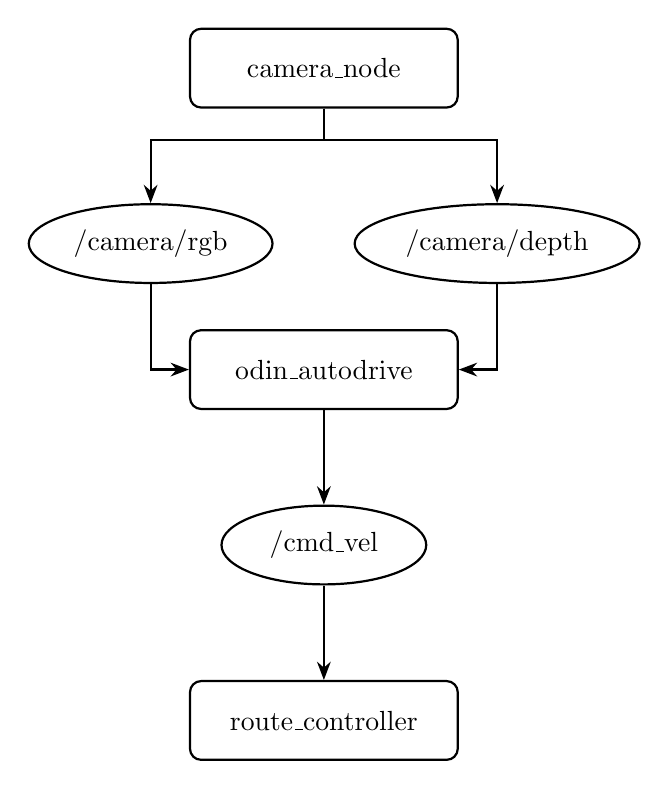
\begin{tikzpicture}[
        node distance=1.8cm and 2cm,
        box/.style={rectangle, draw, rounded corners, minimum width=3.4cm, minimum height=1cm, align=center},
        topic/.style={ellipse, draw, minimum width=2.6cm, minimum height=1cm, align=center},
        >=Stealth, thick
    ]

    % Camera node
    \node[box] (camera) {camera\_node};

    % Topics under the camera
    \node[topic, below=1.2cm of camera, xshift=-2.2cm] (rgb) {/camera/rgb};
    \node[topic, below=1.2cm of camera, xshift= 2.2cm] (depth) {/camera/depth};

    % odin_autodrive
    \node[box, below=2.8cm of camera] (autodrive) {odin\_autodrive};

    % Command topic
    \node[topic, below=1.2cm of autodrive] (cmdvel) {/cmd\_vel};

    % Route controller
    \node[box, below=1.2cm of cmdvel] (route) {route\_controller};

    % Arrows camera -> topics
    \draw[->] (camera.south) -- ++(0,-0.4) -| (rgb.north);
    \draw[->] (camera.south) -- ++(0,-0.4) -| (depth.north);

    % Arrows topics -> autodrive
    \draw[->] (rgb.south) -- ++(0,-0.3) |- (autodrive.west);
    \draw[->] (depth.south) -- ++(0,-0.3) |- (autodrive.east);

    % autodrive -> cmd_vel
    \draw[->] (autodrive.south) -- (cmdvel.north);

    % cmd_vel -> route_controller
    \draw[->] (cmdvel.south) -- (route.north);

    \end{tikzpicture}
    \caption{Grafo ROS2 dei nodi e dei topic utilizzati nel sistema di navigazione.}
    \label{fig:ros2-graph}
\end{figure}

\input{chapters/results.tex}
\section{Future Works}
\label{sec:future-works}

Sebbene i risultati ottenuti rappresentino un avanzamento significativo nella
navigazione autonoma per rover lunari basati su Reinforcement Learning, esistono
numerose possibilità di estendere il lavoro svolto sia dal punto di vista del sistema di
percezione, sia dal punto di vista del controllo e della cooperazione multi–robot.
Di seguito vengono discusse le direzioni principali per sviluppi futuri.

\subsection{Estensione a piattaforme umanoidi o quadrupedi}

L’architettura sviluppata in questa tesi, pur essendo applicata a un rover a quattro
ruote, è concettualmente compatibile con robot umanoidi o quadrupedi, i quali devono 
affrontare sfide ancora più complesse in termini di bilanciamento, percezione attiva 
e locomozione su terreni irregolari.

Negli ultimi anni, vari lavori hanno mostrato come policy basate su RL profondo siano in
grado di controllare gaits altamente dinamici su robot quadrupedi come ANYmal
\cite{lee2020learning, hwangbo2019learning} o su umanoidi di nuova generazione
\cite{xia2022learning}.  
L'adattamento della pipeline sviluppata in questa tesi a tali piattaforme
permetterebbe:

\begin{itemize}
    \item di combinare percezione locale e controllo dinamico, integrando stima della
          pendenza e clustering del terreno con locomozione reattiva;
    \item di testare la robustezza della pipeline percettiva a condizioni cinematicamente
          complesse (rotazioni rapide del torso, oscillazioni dei sensori, ecc.);
    \item di studiare politiche attive di percezione, in cui il robot muove il corpo per
          acquisire osservazioni migliori.
\end{itemize}

L’integrazione con robot come ANYmal sarebbe inoltre particolarmente indicata per
missioni lunari o marziane dove è necessario superare ostacoli impossibili per un rover
tradizionale.

\subsection{Policy collaborative per mappatura e navigazione cooperativa}

Un’estensione naturale del lavoro riguarda l’impiego di più robot che condividono
informazioni tra loro al fine di migliorare sia la mappatura che la navigazione.
Nel contesto del RL multi–agente, diverse architetture collaborative hanno dimostrato
di migliorare l’esplorazione e ridurre l’incertezza del terreno, tra cui:

\begin{itemize}
    \item \textbf{QMIX} \cite{rashid2018qmix}, un metodo di value decomposition per
          coordinamento decentralizzato;
    \item \textbf{MADDPG} \cite{lowe2017multi}, particolarmente adatto ad ambienti
          continui e cooperativi;
    \item \textbf{MAPPO} \cite{yu2022surprising}, oggi lo standard per scenari
          multi–robot complessi con politiche centralizzate durante l’addestramento e
          decentralizzate in esecuzione.
\end{itemize}

L’utilizzo di più rover dotati della pipeline di percezione proposta in questa tesi
permetterebbe di:

\begin{itemize}
    \item ampliare la conoscenza del terreno tramite \textit{shared local mapping};
    \item ridurre l’incertezza di classificazione delle pendenze grazie ad osservazioni
          multiple provenienti da angoli differenti;
    \item costruire mappe di rischio con validazione incrociata tra agenti;
    \item coordinare traiettorie sicure, evitando situazioni in cui più robot entrano
          contemporaneamente in zone ad alta pendenza.
\end{itemize}

Tali approcci collaborativi rappresentano un passo chiave per missioni lunari in cui
più robot operano simultaneamente su vaste aree inesplorate.

\subsection{Riconoscimento di crateri come ostacoli strutturali}

Uno dei limiti della pipeline attuale è l’incapacità di identificare crateri profondi,
che costituiscono una classe di ostacoli significativamente diversa rispetto alle
pendenze positive.  
Il rilevamento dei crateri è noto essere un problema complesso: lavori recenti mostrano
che i metodi tradizionali basati su edge-enhancement e template matching non sono
sempre affidabili \cite{silburt2019lunar}, mentre modelli di deep learning per negative
obstacle detection si sono dimostrati efficaci su robot terrestri
\cite{macenski2020neural}.

Essendo i crateri caratterizzati da \textit{slopes negative}, un’estensione naturale
della pipeline potrebbe comprendere:

\begin{itemize}
    \item una fase di clustering dedicata alle regioni depresse della point cloud;
    \item un modello RANSAC invertito per stimare superfici concave;
    \item l’integrazione di feature geometriche su scala più ampia;
    \item una reward function che penalizzi l’avvicinamento a depressioni ad alto
          gradiente negativo.
\end{itemize}

L’identificazione robusta dei crateri risulterebbe essenziale per garantire la
sicurezza del rover in scenari reali.

\subsection{Aggiunta di una seconda camera per migliorare percezione e robustezza}

Attualmente il rover è equipaggiato con una singola camera RGB-D posta a circa
20\,cm dal suolo, il che limita notevolmente:

\begin{itemize}
    \item la distanza massima di percezione;
    \item la capacità di identificare crateri e variazioni profonde del terreno;
    \item la robustezza alla perdita temporanea di informazione dovuta al rumore.
\end{itemize}

Una possibile estensione consiste nell’aggiunta di una seconda camera montata più in
alto, come suggerito da diverse ricerche sulla percezione multi-view
\cite{zhou2018stereo}.  
I benefici principali includerebbero:

\begin{itemize}
    \item \textbf{sensor fusion} per filtrare il rumore e ottenere misure di profondità
          più stabili;
    \item \textbf{maggiore look-ahead distance}, fondamentale per anticipare ostacoli
          e pianificare traiettorie più sicure;
    \item \textbf{capacità di individuare crateri}, poiché l’angolo di vista
          dall'alto migliorerebbe la percezione di depressioni nel terreno.
\end{itemize}

L'integrazione di due camere richiederebbe una pipeline di calibrazione e fusione
(in stile extrinsic + depth fusion) ma permetterebbe un miglioramento sostanziale
rispetto alla configurazione attuale.


\input{chapters/real_results_campaign.tex}

% -------------------------------
% BIBLIOGRAPHY
% -------------------------------
\bibliographystyle{ieeetr}
\bibliography{reference}

\end{document}
